\textbf{Camp \emph{X-Ray} (-550 m): Inside the Hollow Mountain}


\textbf{Sledi Vetra 2012}

\textbf{11:45 Weds 18/7/2012 Jonny}

Back in underground camp one year later!\\
A smooth trip down, everything has now been de-moulded in camp. Tea
ready, about to cook.. It's good to be back!

\textbf{Niko}

Finally back in camp \emph{X-Ray}, mental! Last time I was here two
years ago. Journey here was generally alrite, just Jonny sort of started
leaving tace sacks as he started rigging, so more load 4 us, but he did
a good job rigging. \emph{Zimmer} annoying. Camp was quite mouldified,
but Jonny covered with sand. Cooking now, everything is alrite.
Definitely less rapture than 2 years ago. I just sort of thought that
it's a pretty unique situation here. Cos normally whatever youre doing
in life (eg smoking weed) there must be a lot of people at that same
instant around the world doing the same thing, but I think at this
moment, we are very likely the only people in this world living in a
deep underground camp, like us. Crazy thought. We are truly alone.
Waiting for cous cous. Everything is alrite. So yea, Camp \emph{X-Ray}
2012 is again in operation. Enjoy!

\textbf{Oli}

Gone down more pitches than I can remember.. Underground camp is
actually much warmer than I thought it would be. Time for dinner --
Ainsley Hariets cous cous.

\textbf{1:47 am Friday 20\textsuperscript{th}} \textbf{July Rhys}

Nice easy trip down to camp. Left at sunset, down for about midnight.
Have eaten cous cous, smash and sausage. I don't know what I thought
camp would be like but I'm here and I like it. Hopefully shall have nice
long sleep.

\textbf{2:30 a.m. 20/7/2012 Tetley}

Back at \emph{X-Ray} -- the 4\textsuperscript{th} year we've had a camp
here ('03, '10, '11, '12). Rhys and I had a smooth journey down -- now
drinking Žganje and listening to Blackadder. Now some sleep!

\textbf{11:40 a.m. 20/7/2012 Tetley}

A decent kip, slight headache though. I'm thinking of tea, and the
pushing front.

\textbf{12:47 p.m. 20/7/2012 Rhys}

Sleeping was good, camp is comfy. Breakfast soon, yum. Really excited
about pushing. Where else can you doss about in the sun one day and be
at the limit of human exploration the next day? Its going to be good.

\textbf{2:40 p.m. 20/7 Tetley}

The classic `Cheesy, soupy, fishy smash' for breakfast. Almost finished
packing food, brew kit, bolting kit, rigging kit, survey kit. Had a
shit. Cup of tea then time to put caving kit on\ldots{}.

\textbf{Tet}

It's 20 dedgree Celcius down here -- or so says the thermometer I bought in
Tolmin! Dr.~Tim, a rubber chicken (and Samo's pants!) are watching over
us!

``It's not just about the pushing, it's also about the journey.''

``Yeh''

\textbf{3:50 pm 20/7 Tet}

Rhys and I are finally heading off to Salvation. Back by 8 a.m. at the
latest.

\textbf{4:10 pm 20/7 Clare}

Good trip down with Jarv, great to be back at \emph{X-Ray}! Nothing's
changed, it's like coming home. Had a quick chat with Tet and Rhys just
as they were leaving to push Salvation. We will be off to kill Winters
Journey and derig the \emph{Insomnia}/\emph{Daydreamers} series. May
also check out Red Cow and Strap in the Nitro. Expect to be back 9am on
21/7, callout noon.

\textbf{4:15 pm Jarv}

Great to be back! Off to kill the deep stuff.

\textbf{21-7-12 6} \textbf{AM} \textbf{Jarv}

Back!

Pushed: PERFIDIA, a tight dry alternative to \emph{Republika} (pitch).
We were hoping for a Red-Cow sump bypass.

Then went to the bottom \& pushed WATERSHIP DOWN from beyond
WinterJourney.1 (where Fratnik \& Jim opted not to squeeze) down a
{[}STUPIDLY{]} freeclimbed slope to a beautiful deep static sump.

The cave is thus deeper -- perhaps 20-30 m so.

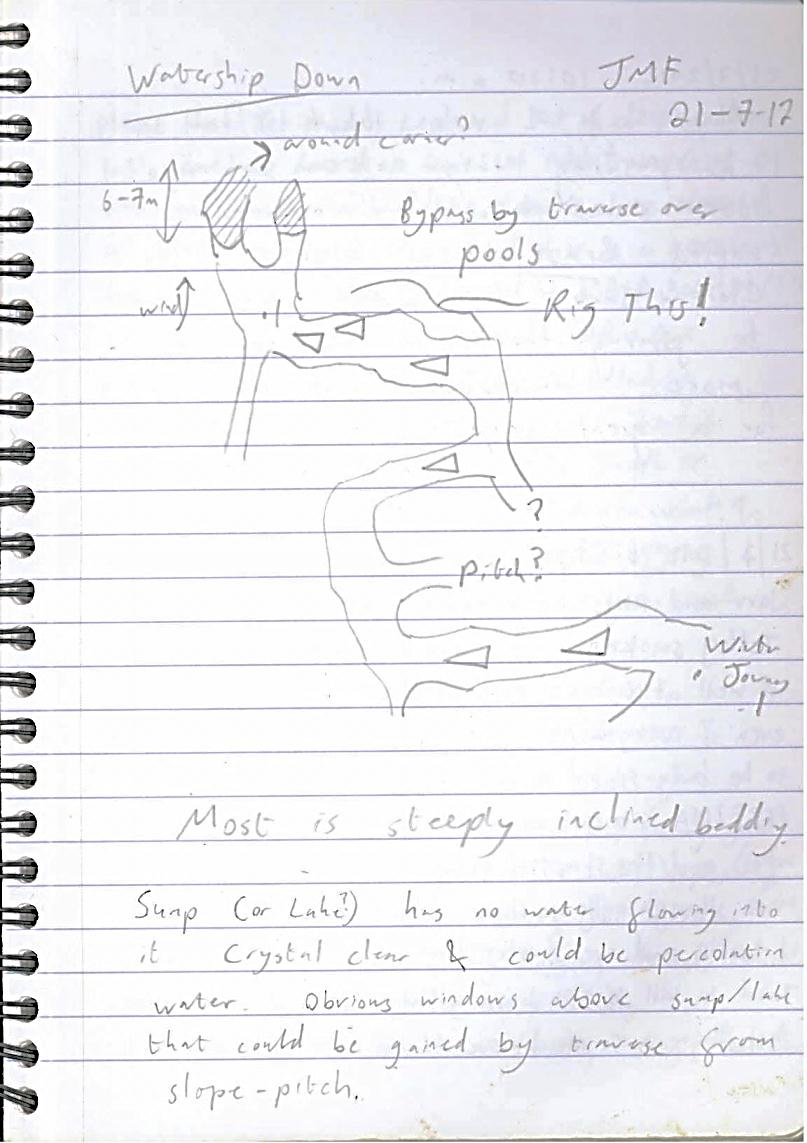
\includegraphics{appendices/ug_logbook/63.jpeg}\\
{[}Jarv's sketch of Watership Down{]}

Most is steeply inclined bedding.

Sump (or Lake?) has no water flowing into it. Crystal clear \& could be
percolation water. Obvious windows above sump/lake that could be gained
by traverse from slope-pitch.

\textbf{21/7/2012 10:10 a.m. Tetley}

Rhys and I are back from a 17 hr pushing trip - approx 100 m in the book. Cave
beyond Salvation named Brave **** New **** World. Clare + Jarv in bed,
we'll soon be joining them in the tent -- more tomorrow. Thanks Rhys for
a great trip!

\textbf{21/7/2012 6:57 pm Clare}

Jarv and Rhys are asleep on either side of me, Tetley smoking a fag in a
corner of the tent -- all is well at Camp \emph{X-Ray}! Excellent push
yesterday, even if everything we found (\textasciitilde 150 m total?)
seemed to be body-sized or smaller!

PERFIDIA is a cool connection between Red Cow (pitch rope) and the start
of \emph{Insomnia}. Saves a fair bit of time, though only go there if
you aren't carrying lots of tackle and are shorter than Jarv!

Tried to kill Winter Journey but it won't die. Amazing that there is so
much cave off an abandoned bedding plane that Tet and I explored out of
desperation last year! We found a series of rabbit warrens -- little
crawlways at a bedding plane incline. Named it WATERSHIP DOWN. At the
end of it is a gorgeous terminal sump (or lake?). Named it MALA BOHIN
(?? Whatever that famous lake is called). Still a few unexplored leads
in Watership down, including what looks like a pitch. Take some rope.
There is loads at Red Cow Roundabout, and a length or two at the start
of Penguin's Egg. If you want to get down to the sump, I'd recommend
rigging a rope down the final slope -- I'd have been stuck there if not
for Jarv to stand on!

Right, going to try and grab more shut eye.

\textbf{11:36 pm 21/7/2012 Rhys}

Just woke up from 12 hour sleep, feeling good. Camp is nicer with 4
people. Tea now, hopefully breakfast soon. Selective memory has already
turned yesterday from mostly slogging through \emph{Penitence} and Stuck
in Paradise to an amazing trip.

At end of Salvation we (mostly Tetley) hammered our way through squeeze
to cool chamber and then Tetley entombed himself digging into boulder
choke. This eventually led to weird streamway. Very drafty all the way!
Definatley two leads up and down streamway. New discoveries called Brave
New World. Looking forward to going back.

\textbf{21-7-12 11:47 PM (says my watch -- feels like 10 AM) Jarv}

Fairly cool night (buf + a fleece liner with an irritating feet-sized
hole in the bottom. Legs kept on cramping -- it's a lot of exercise to
the new new bottom of the cave.

No nightmares about not being able to climb back up from Watership
Down.1 In fact I didn't dream much at all. Just daydreamed of the
beautiful sump \& the crystal clear water.

You wake after a push \& rub the mudstone-sleep out of your eyes, sore
knees, stiff muscles \& odd bruises in strange places. Hmm, anyway --
back to the cave.

Perfidia, the attempted Mad Cow Sump Bypass

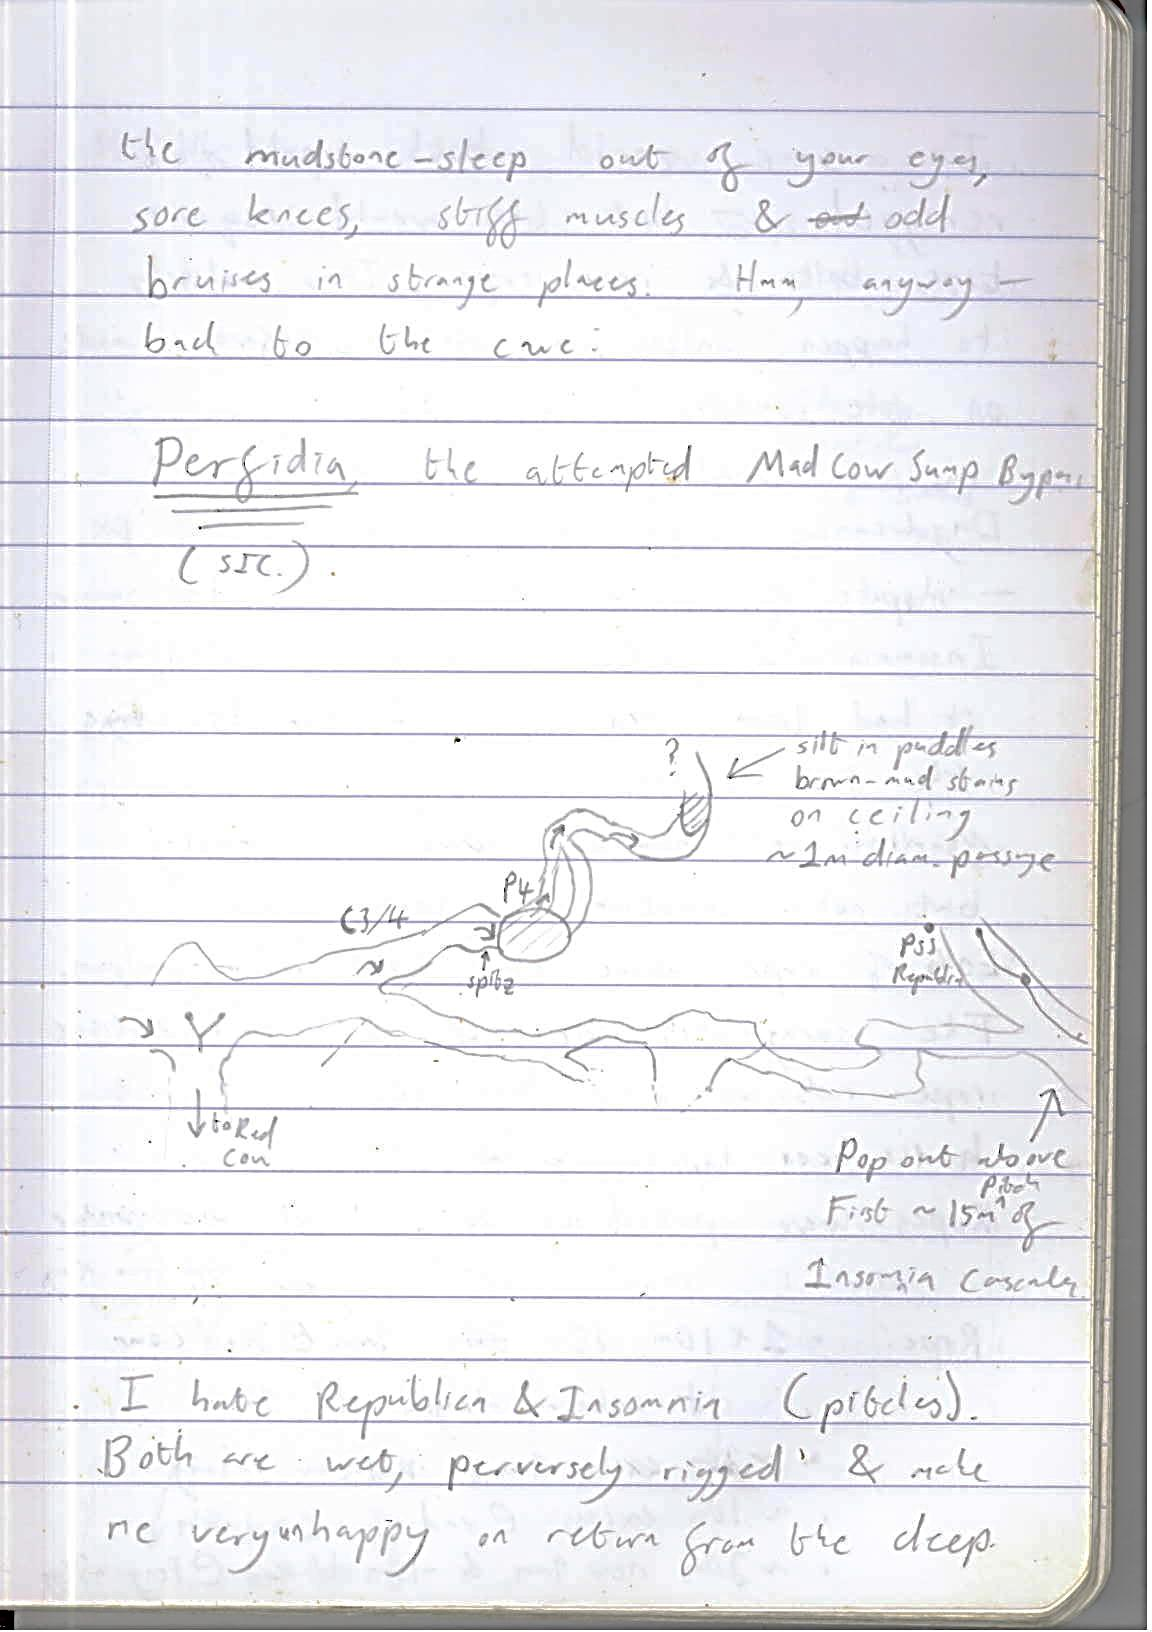
\includegraphics{appendices/ug_logbook/64.jpeg}\\
{[}Jarv's sketch of Perfidia{]}

I hate \emph{Republika} \& \emph{Insomnia} (pitches). Both are wet,
perversely rigged \& make me very unhappy on return from the deep. In a
sane world both would be rerigged -- but this would require time, bolts
\& new rope. Thus unlikely to happen unless a serious effort is made on
the sumps.

\emph{Daydreamers} rope was actually all OK -- inspite of being left
rigged last summer. \emph{Insomnia} I had to reverse prussic as it had
been tied off (I suspect) by the last climber last year.

Maillons in Dreamers were v.rusty but not structurally so.

Ends of rope where cut had been pulped. The swing-pitch above the pool
had extreme rope rub on where the horizontal section had been
tap-tapping on the floor. Ropes were pulled up \& tied off were
possible.

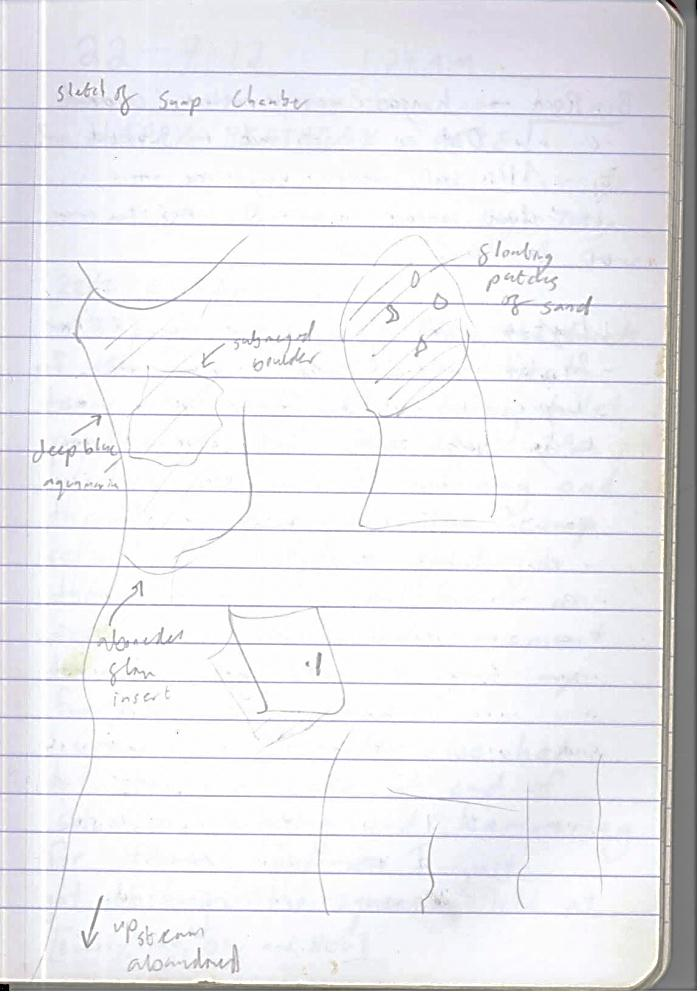
\includegraphics{appendices/ug_logbook/65.jpeg}Rope:

\begin{itemize}
\item
  1 x 10 m, 15 m, 20 m 9 mm @ Red Cow (taken from \emph{X-Ray} on this
  trip) + unknown-length old 9 mm
\item
  approx 20 m excess 9 mm on Red-cow Y-hang
\item
  approx 10 m excess @ end of \emph{Insomnia}
\item
  approx 20 m new 9 mm approx 15 m old 9 mm @ Penguin's Egg
\end{itemize}

Big Rock -- hangers were rather corroded. Didn't like it much --
substitute soon? All bolts were very loose -- does someone come \&
loosen them over winter? Odd.

Left a few dirn. arrows for Red Cow \& back to Big Rock (as far as
Leprecaun pitch) Not sure if they help much, but we do try\ldots{}

{[}Jarv's sketch of sump chamber{]}

\textbf{22-7-12 1:24} \textbf{AM} \textbf{Clare, Rhys, Tetley \& Jarv}

HAPPY BIRTHDAY PETE!

\textbf{22/7 2:18} \textbf{am} \textbf{Tetley}

3 pages are missing from the back of this logbook\ldots{}. The first
team down forgot to bring toilet paper. Apparently the paper I'm writing
on is soft, strong and thoroughly absorbent! The camp setup team* did a
great job though, \emph{X-Ray} is as homely as ever, too nice at the
moment to make me want to put my furry on too soon.

{[}*Jonny, Mike, Olly and Nico{]}

Great trip yesterday, we had hot tea and cake at end of Salvation.
Digging and hammering for 40 mins, and I just got through the squeeze
left at the end of last year's expo.

Back in new territory. More digging and hammering enlarged the squeeze.
Rhys and I were now in a small chamber. Wind so loud through squeeze it
sounds like the roar of a stream.

Damn, no way on, big boulder choke. Wait\ldots{} maybe up there,
no\ldots{} yes\ldots{} hanging death above. Tried to dig up but scary
boulder led to a change of tactics, went right, horizontal, under said
boulder. Scary digging up, but I had the draught and could see big
passage above\ldots{}.

Soon I had a hole large enough to squeeze through. Told Rhys to smoke
all my tobacco if I should die and went for it. Crash. Collapse, I was
trapped. Well past the point where rescue is possible\ldots{} Could just
move left hand\ldots{} slowly, with the help of Rhys, I dug myself out
and we were through.

Its true to say that we weren't in the huge, horizontal passage with
stals and gour pools that I'd dreamed about. But it didn't matter! The
thrill of being in new, unexplored passage never wears off.

Up a slope (crawling) passage gets bigger heading east going up at approx40 deg
to horizontal. We climbed up a slope until passage broke into what looks
like an active streamway (though it only has a tiny trickle of water in
it -- not even enough to collect to drink). Upstream left unpushed,
downstream has the draught! We surveyed approx20 m down stream. Left
draughting bedding plane crawl as the going lead.

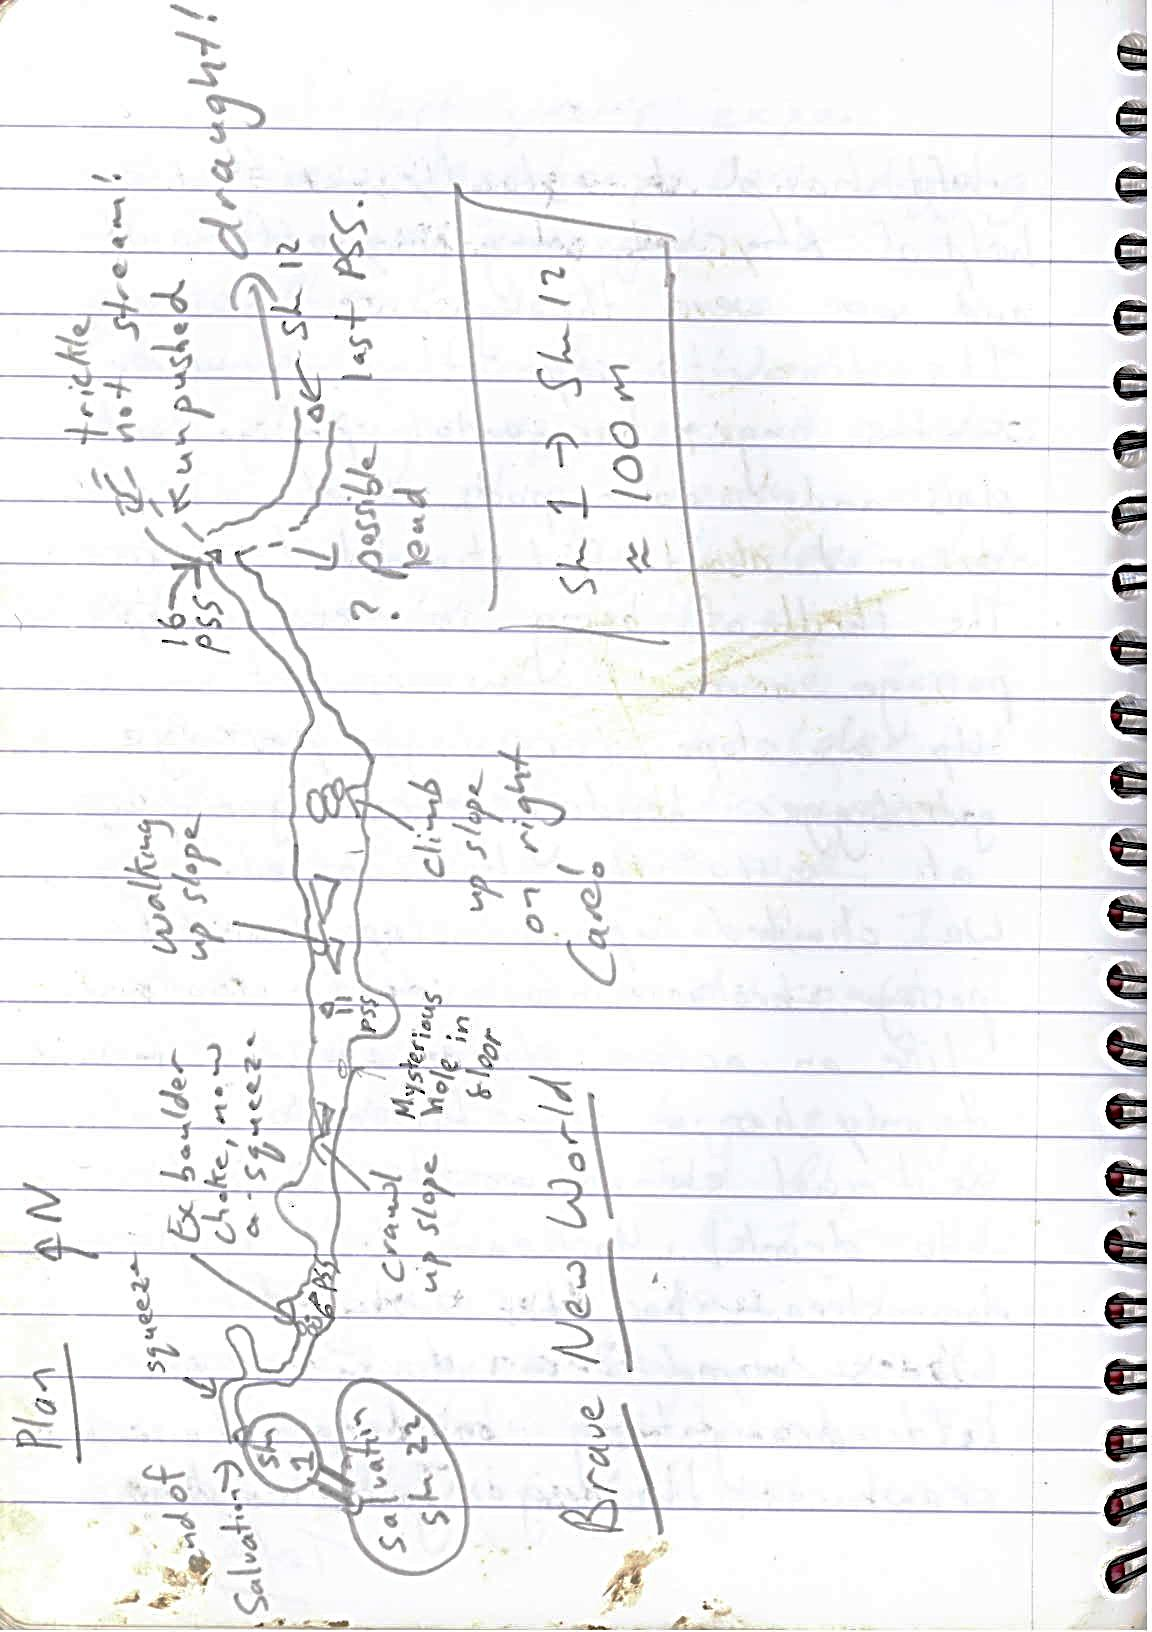
\includegraphics{appendices/ug_logbook/66.jpeg}{[}Tetley's sketch of \emph{Brave New
World}{]}

\textbf{22/7/2012 5:20 am Clare}

Clare + Jarv off to push Throne Room. Expect to be back by 2pm.

\textbf{22/7/12 6 a.m. Tetley + Rhys}

We've found Xanadu!

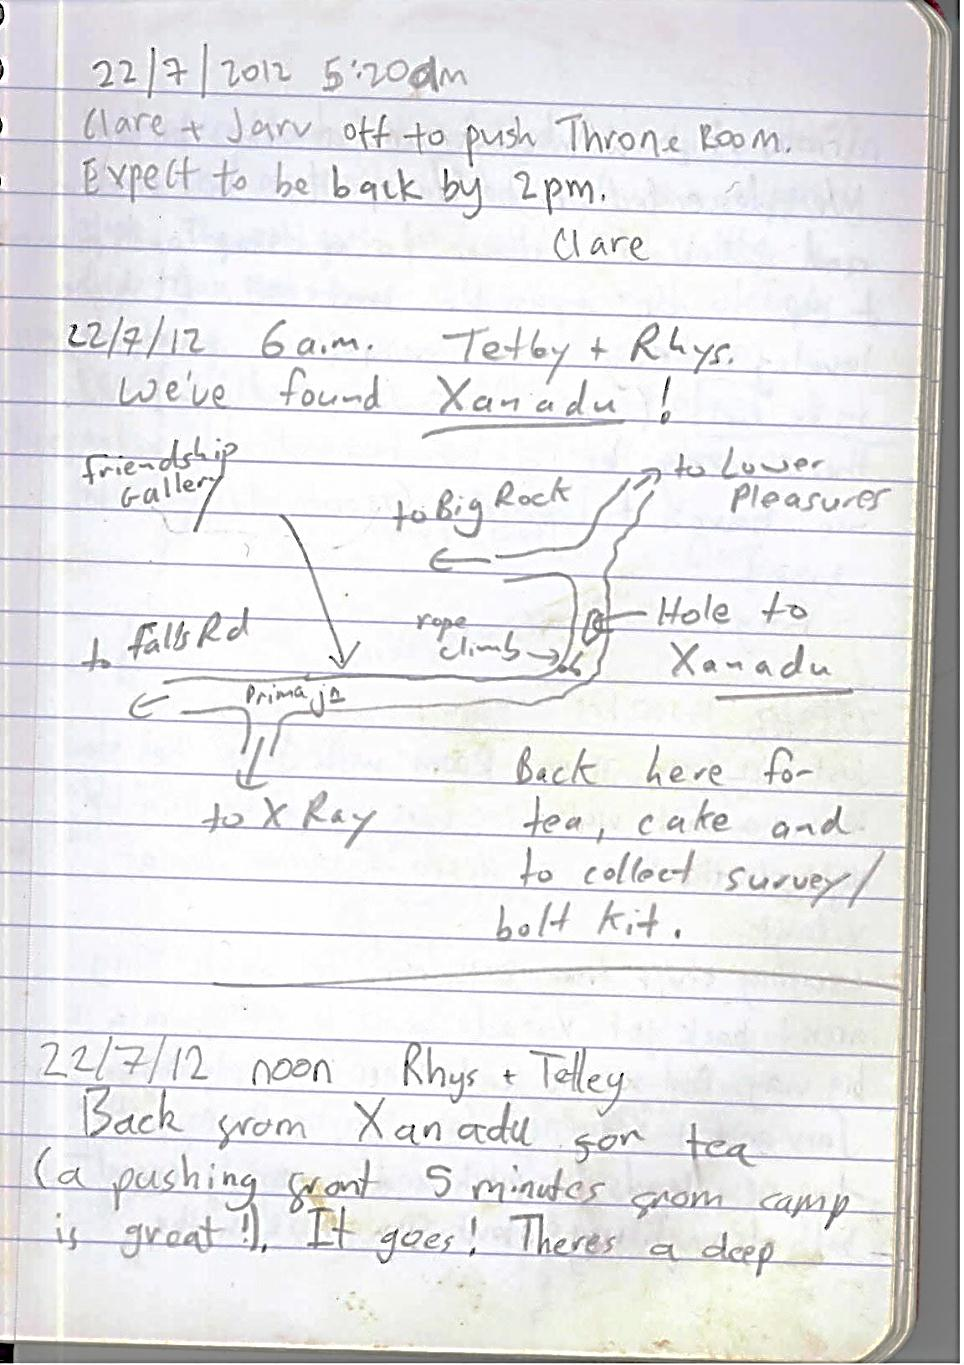
\includegraphics{appendices/ug_logbook/67.jpeg}\\
{[}Tetley's directions to Xanadu{]}

\textbf{22/7/12 noon Rhys + Tetley}

Back from Xanadu for tea (a pushing front 5 minutes from camp is
great!). It goes! Theres a deep narrow rift with a stream at the bottom.
We descended right down to the stream and followed it down to a sump and
followed it up to an impassable waterfall. At higher levels in the rift
we may have found a sump bypass (going to explore that now) and there
may be a waterfall bypass but we haven't looked. Great trip so far!

\textbf{22/7/12 14:00 hrs Clare}

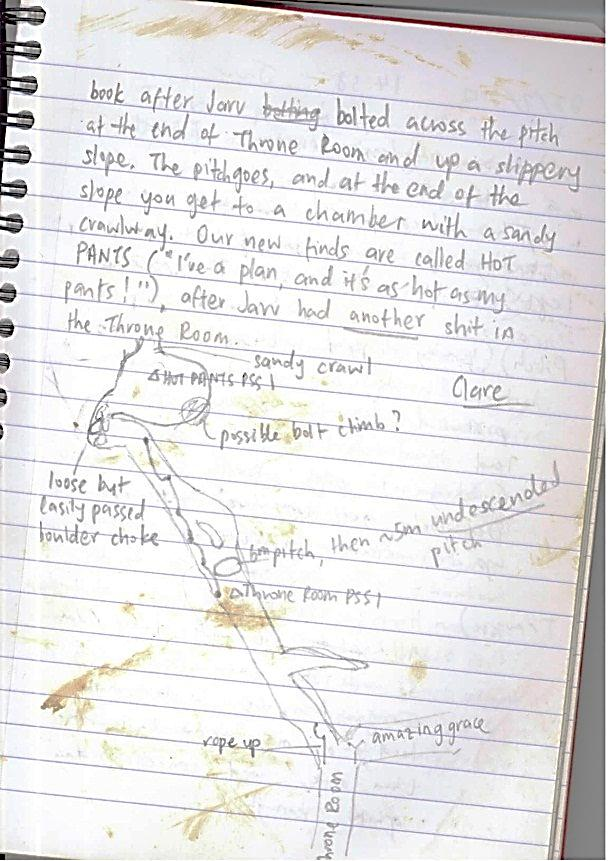
\includegraphics{appendices/ug_logbook/68.jpeg}Just back from Throme Room with Jarv;
he's having a shit, water for cous cous is heating up, Night of the
Proms on stereo -- another day at \emph{X-Ray}!

Exciting stuff from Rhys and Tet above! They aren't back yet, Xanadu
must be going in a big way. And so the leads keep multiplying\ldots{}.
Jarv and I returned from Throne Room with two new leads: a pitch and a
sandy crawl -- both draughting. About 50 m more in the book after Jarv
bolted across the pitch at the end of Throne Room and up a slippery
slope. The pitch goes, and at the end of the slope you get to chamber
with a sandy crawlway. Our new finds are called HOT PANTS (``I've a
plan, and it's as hot as my pants!''), after Jarv had another shit in
the Throne Room.

{[}Clare's sketch of Hot Pants{]}

\textbf{22/7/2012 14:38 Jarv}

Mmm, oil-less couscous. It's been a while.

The Uneo proved its worth again attacking the two `sort of leads' we
left at the end of the Throne room.

Pitch) Easily dropped with bolt on large boulder \& tackle-bag rub
protected descent. Crawl opposite lead immediately to \textasciitilde 4
m draughting (sucking in) pitch. Possibly free climbable. Definitely
goes somewhere, I returned up to attend the traverse.

Traverse) Horrific to bolt. Rock v. dodge. All foot holds loose/dubious.
So much shit came down/on me. I found myself unintentionally landing on
my cows-tails more than once, and once a day is quite enough.

Traverse proceeds up 60 deg inclined slope of death. Minimally gardened to
avoid slicing rope. Top section is a jammer/abseil section that goes
over a massive pile of boulders, extreme care \& possibly a rebelay bolt
required.

From top of traverse (phew!) careful climb up slope \& through boulder
choke to a fairly impressive chamber \textasciitilde 7+m high with
passage leading of at about \textasciitilde 4 m above floor.

More importantly, a crawl goes from the edge of the chamber blowing into
your face over a white mud/stone blockage that is easily diggable (Clare
just slipped over). Apparently it continues on \& on. Perhaps ideal for
the small wrigglers amongst us.

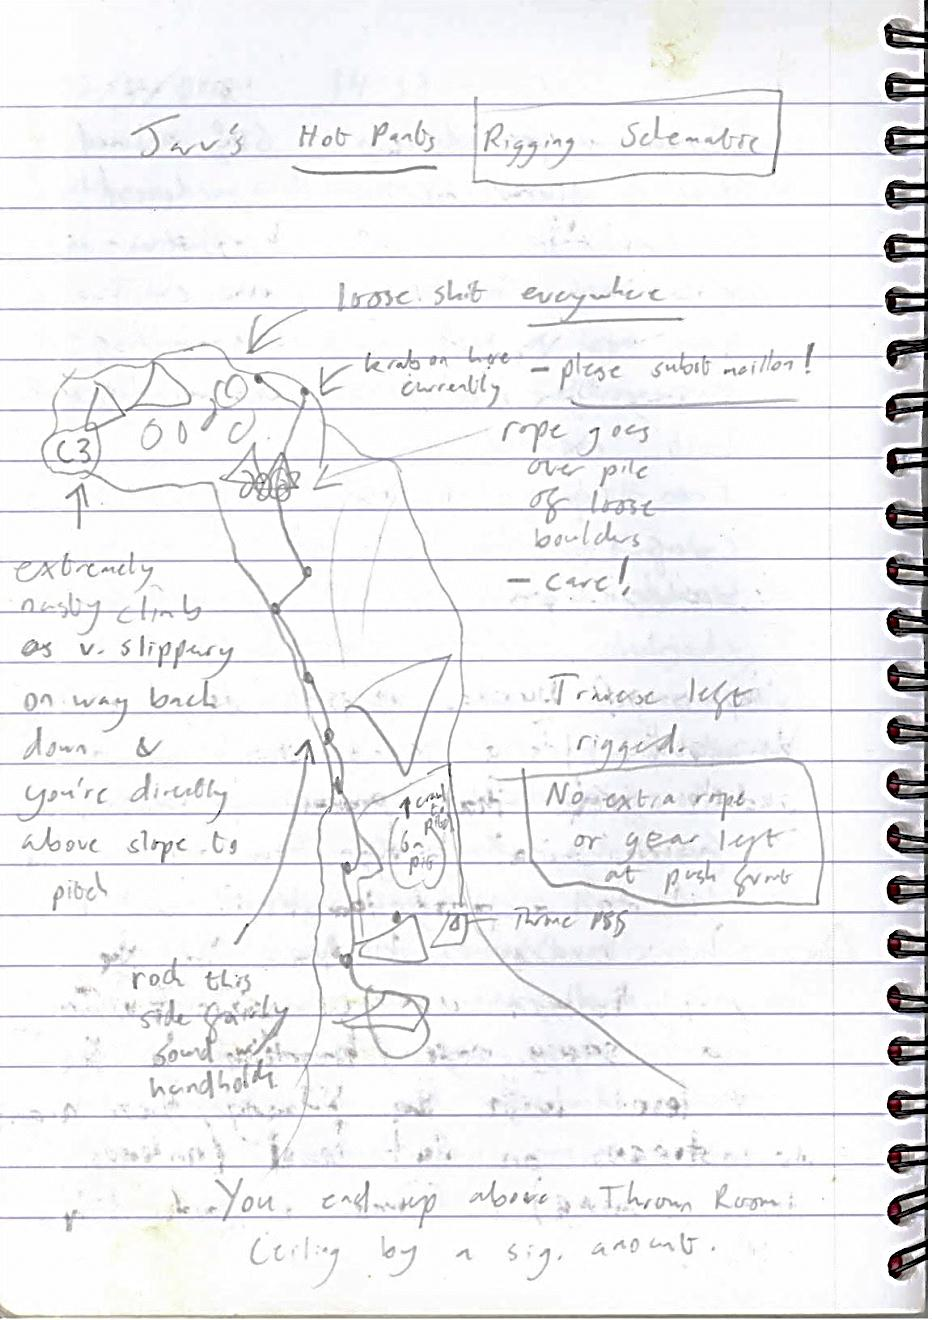
\includegraphics{appendices/ug_logbook/69.jpeg}\\
{[}Jarv's Hot Pants Rigging Schematic{]}

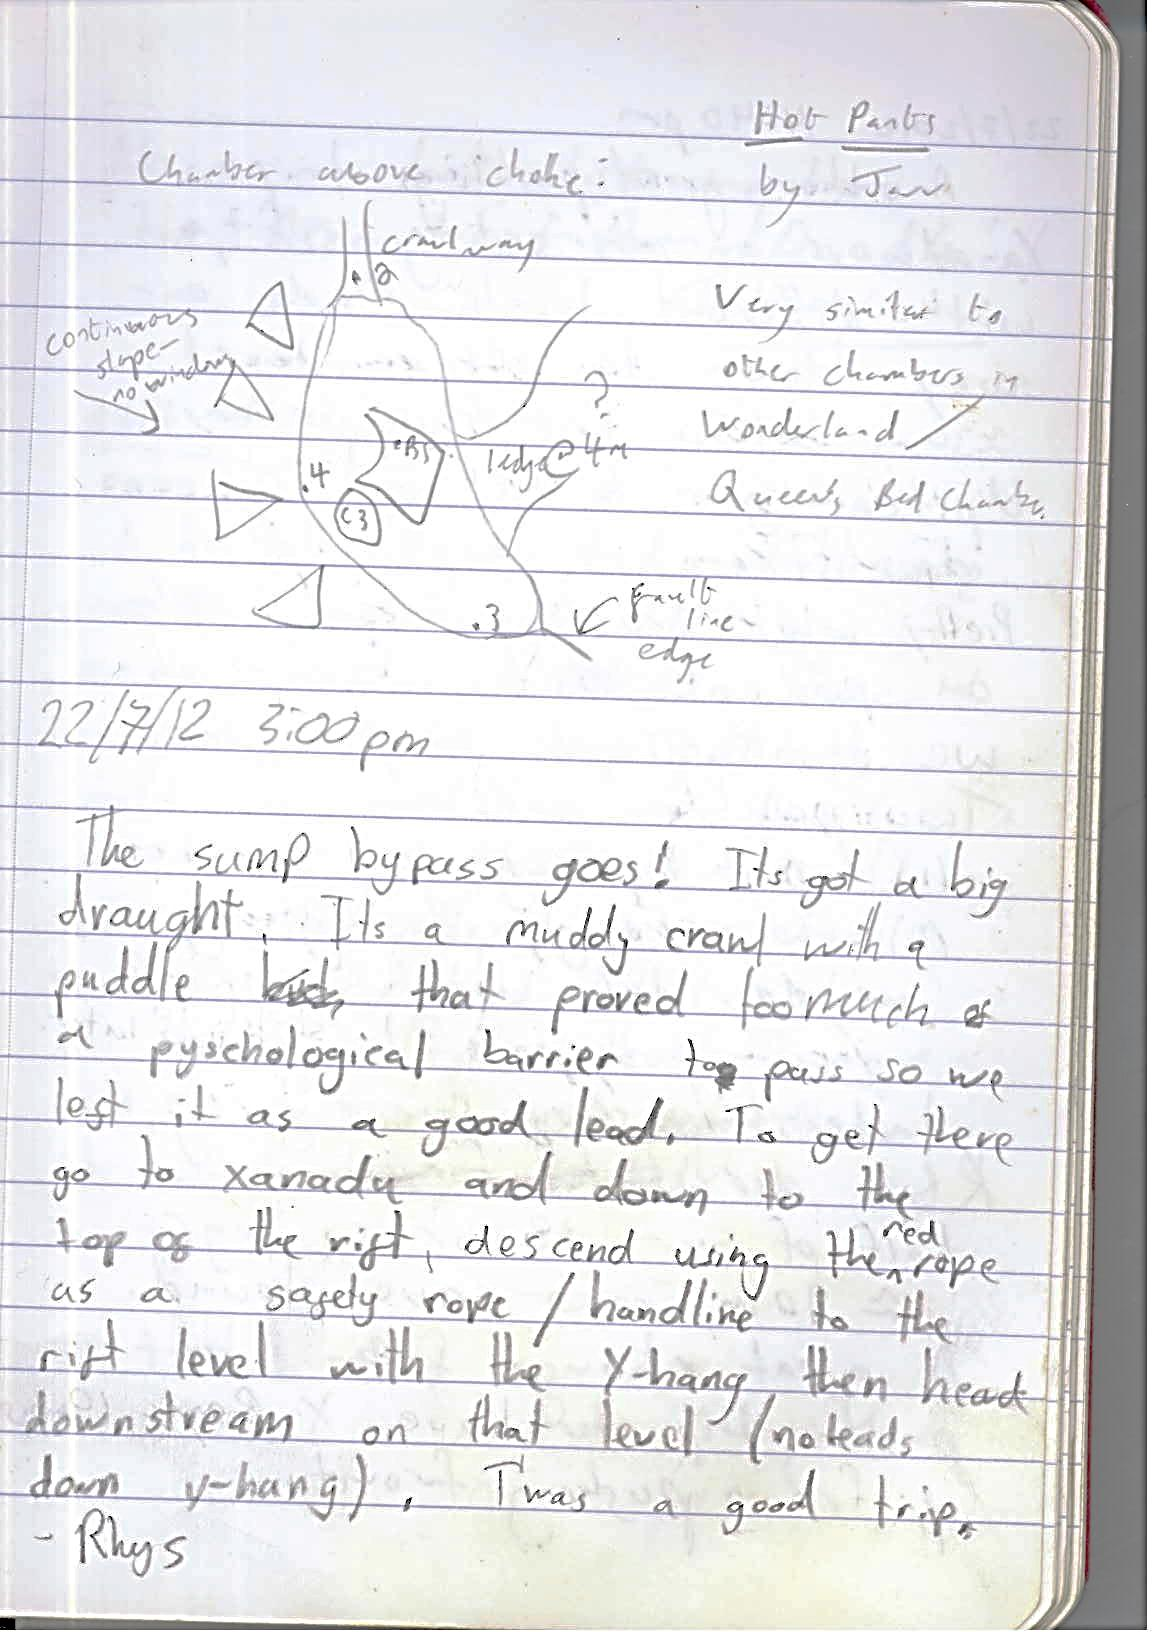
\includegraphics{appendices/ug_logbook/70.jpeg}\\
{[}Jarv's sketch of Hot Pants chamber{]}

\textbf{22/7/12 3:00 pm Rhys}

The sump bypass goes! Its got a big draught. It's a muddy crawl with a
puddle that proved too much of a psychological barrier to pass so we
left it as a good lead. To get there go to Xanadu and down to the top of
the rift, descend using the red rope as a safety rope/handline to the
rift level with the Y-hang, then head downstream on that level (no leads
down y-hang). T'was a good trip.

\textbf{22/7/2012 4:40 pm Tetley}

Another great pushing trip. Xanadu is an interesting rift, with
different levels. Made our way down to stream level approx 30 m below
Friendship Gallery. Upstream goes to a wet squeeze, downstream to a
sump. Pretty white rock, lovely ripples on pool of water, found what we
think is a sump bypass. Two possible leads --

\begin{enumerate}
\def\labelenumi{\arabic{enumi}.}
\item
  Push up high up stream
\item
  The strongly draughting muddy tube with puddle (sump bypass?) --
  sketch to follow later
\end{enumerate}

Interesting surveying, Rhys did book for half of our 18 or so legs. approx 90
m new cave found. A great change from last pushing trip to have
\emph{X-Ray} 10 mins from pushing front. Now in bed, listening to `the
Ascent of Run Doodle'.

\textbf{22/7 8:50 pm Tetley}

3 hours of (Žganje induced?) sleep and I'm awake again. No sign of a day
train\ldots{}. One would be good on the deep pushing front but bad for
me, don't want to get kicked out of bed. On Saturday the stream sounded
pretty loud (but not of the apocalyptic level Jonny and I heard last
year. Now it sounds fairly normal.

\textbf{22/7/12 9:01 pm Clare}

Really should be asleep, but am just on the wrong side of restless to do
so! Fingers crossed the day train doesn't arrive to kick us out of
bed\ldots{} Rhys has just got up for a piss, only to find the piss BDH
full\ldots{} so he promptly went to \emph{Zimmer} to empty it. What a
trooper!

\textbf{23/7/12 1:22 am Rhys}

Sam and Mike have arrived looking for beds. Tetley has used jedi mind
tricks and convinced Clare and Jarv to leave now. More sleep for us then
out I think. I wish I could stay and push more but the surface and
dossing calls.

\textbf{23-7-12 1:34} \textbf{AM} \textbf{Jarv}

Oh no! They're here\ldots{}. Mike \& Sam arrive, in search of comfort
form the storm.

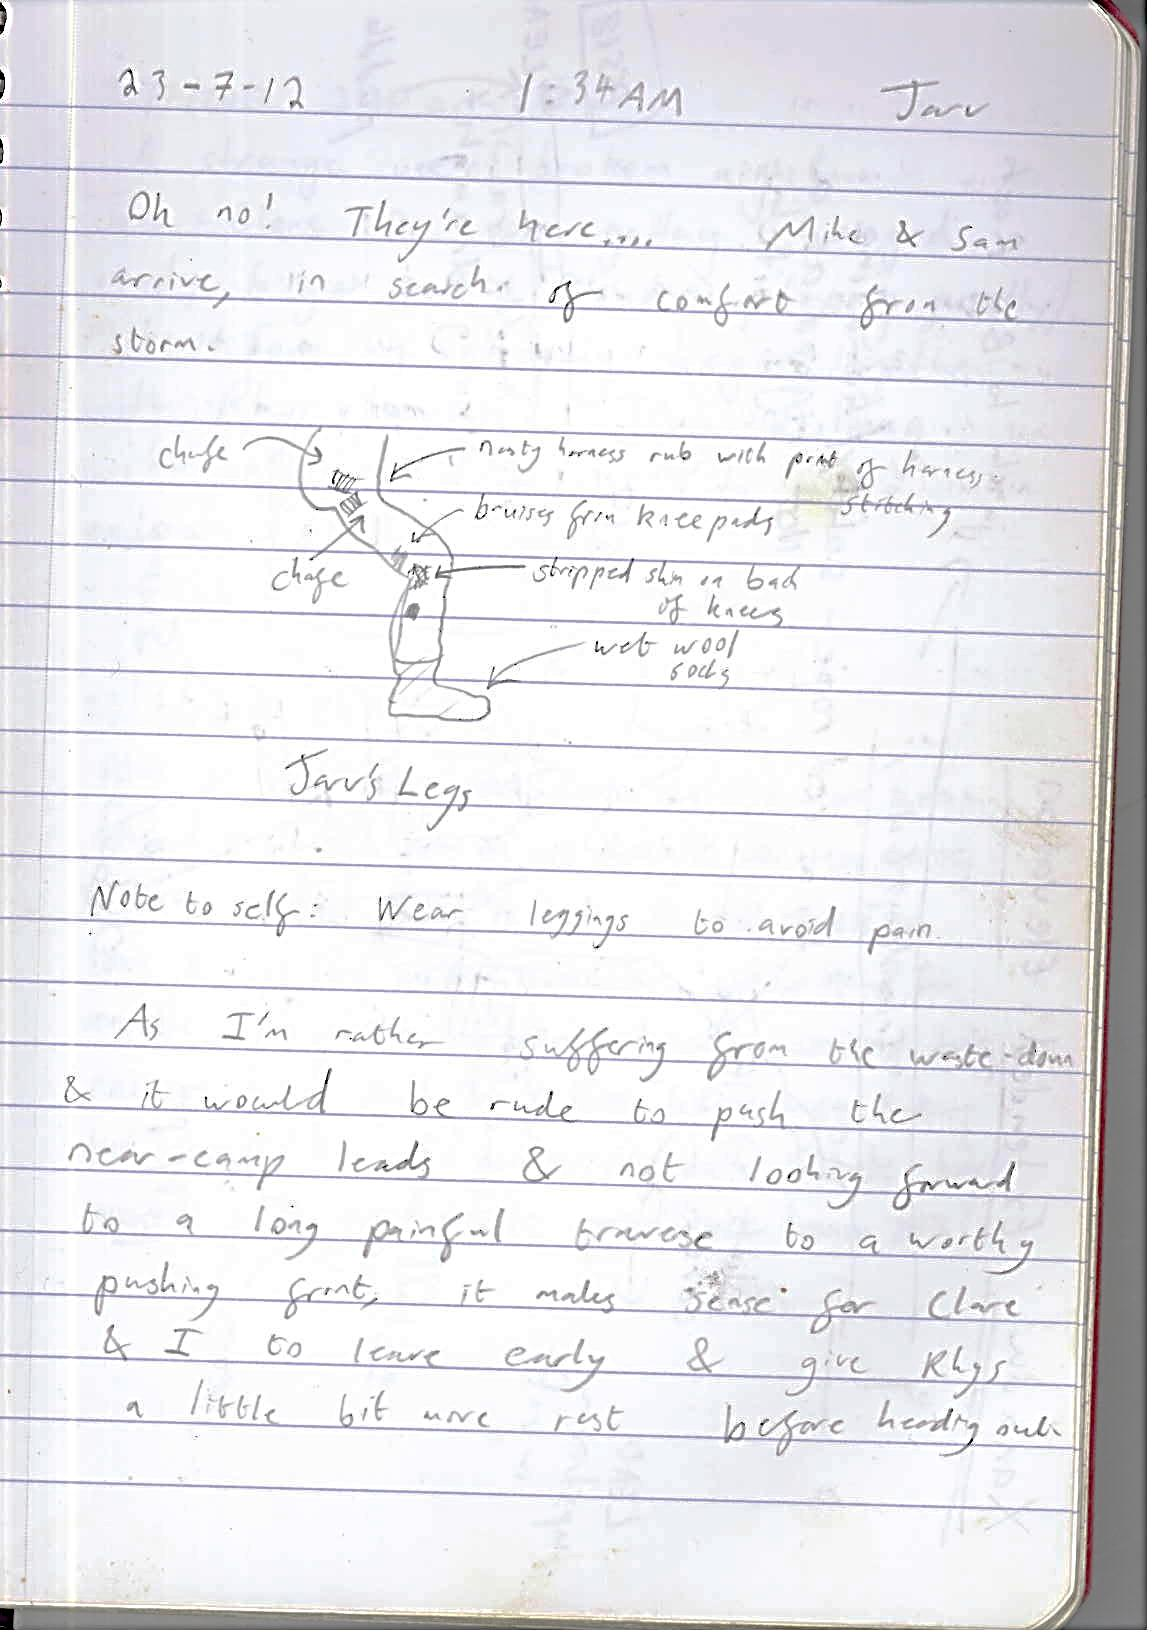
\includegraphics{appendices/ug_logbook/71.jpeg}\\
{[}Jarv's drawing of his chafed legs{]}

Note to self: Wear leggings to avoid pain

As I'm rather suffering from the waste-down \& it would be rude to push
the near-camp leads \& not looking forward to a long painful traverse to
a worthy pushing front, it makes sense for Clare \& I to leave early \&
give Rhys a little more rest before heading out.

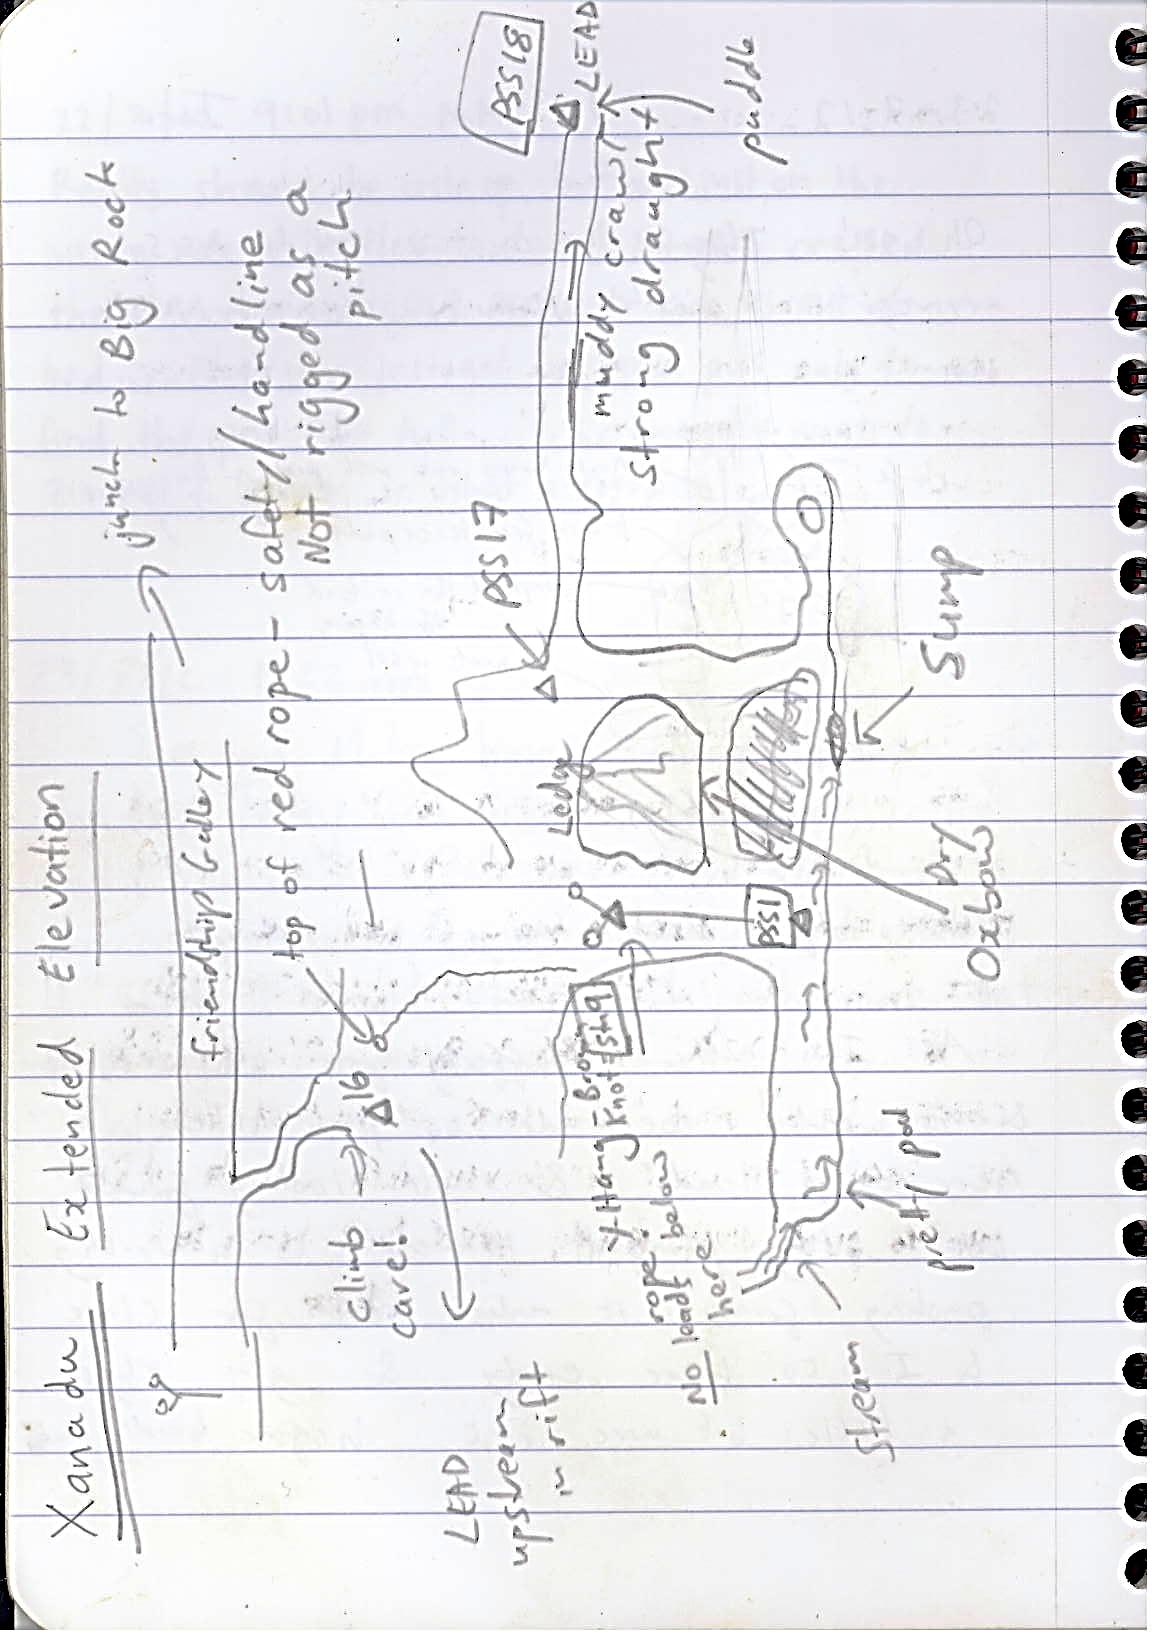
\includegraphics{appendices/ug_logbook/72.jpeg}\\
{[}Tetley's extended elevation sketch of Xanadu{]}

\textbf{23/7/2012 3:30 a.m. Tetley}

A strange very broken night\ldots{}. Jarv + Clare are now getting
changed ready to go out (Blondie playing quietly). Mike + Sam in
sleeping bags, together with Rhys + myself. Jarv drilling with electric
drill\ldots{}.. (to make extra clothes rail).

\textbf{23/7/2012 3:30 am Clare}

Alas, Mike + Sam came down on the day train around midnight, just as we
thought we were going to have another 8 hrs in bed\ldots{} Oh well,
guess we have to hit the surface sometime. Will be good to see the sun
again. It's been a great camping trip, cheers Jarv! And Tet + Rhys for
making \emph{X-Ray} fun. Excited to enter our survey data! Will be back
soon to push more leads, good luck team 2012!

\textbf{Tetley}

Some thoughts on pushing beyond \emph{Brave New World}

\begin{itemize}
\item
  It's a very serious trip -- don't underestimate it, even a club rescue
  might not be feasible, a major injury would be a disaster best to
  think RESCUE IMPOSSIBLE
\item
  Take Water. Rhys + I took 1.5 litres each, this was about right. No
  water in cave from \emph{Zimmer} onwards.
\item
  Recommended: a brew kit, (meths + fish tin). Hot tea and hot fish
  sandwiches went down a treat!
\item
  Allow a minimum of 4.5 hrs each way between \emph{X-Ray} and the
  pushing front.
\item
  \emph{Stuck in Paradise} -- Rhys + I went down and up in sections, one
  at a time, i.e.~I went down to a point where I was safe from falling
  rocks then stayed at rebelay until Rhys joined me, we then repeated
  this. This worked very well!
\item
  On two sections on way down rope had caught around rock/flake so was
  very taut. Down prussiked/Italian hitched down.
\item
  approx 20 m of yellow rope is at top of Stuck in P.
\item
  approx 40 m of rope has been left at end of Salvation.
\item
  Rhys and I had a 17 hr trip.
\item
  Some draught from \emph{Amazing Grace} all the way through to Brave
  New World pushing front. What's driving it????
\end{itemize}

\textbf{23-7-12 03:52 Jarv}

So long \emph{X-Ray}!\\
Another fine 60 hour stay (check-in till check-out).\\
Some great pushing, we've left some good leads -- just treat the Throne
Room traverse \& new deep bits with respect -- they're not as protected
as should be \& rescue from both would be difficult if not improbable.

Off with the camp rubbish \& flat drill batteries, and a too-exciting
mix of methanol \& petrol (that first day in the Bivi mix up still
haunting us).

Safe caving, good luck pushing \& see you again as soon as my sores
heal!

\textbf{23/7/12 9:45 a.m. Tetley}

Rhys and I left the surface 85 hrs ago. Rhys throughout has seemed
utterly unfazed by his first camp, deepest trip, longest days pushing,
caving with me (!) etc. etc\ldots{}. Mike snoring on and off, Rhys + Sam
lying silently in pits. I'm fully awake now, listening to Bach (and
Mike's nose) and drinking tea. This cave and the cavers who push are
truly amazing, the combination of the two is something very special
indeed! It's strange, normally after this much time underground I'm very
keen to see the sun; on this trip, however, I haven't really even
thought about it. Is this a good thing or a bad thing???

\textbf{23/7/12 10:24 am Rhys}

Weird 19 hours in bed, was awake for about 9 hours of it I think. Tetley
making tea. Inevitable trip to surface rolls closer.

\textbf{23/7/12 10:30 am Sam}

Don't think I got a great deal of sleep last night. I was plenty warm
enough\ldots{} but it was difficult to drop off. Perhaps because of
Mike's snoring? Anyway camp is a pretty cool place, and I don't feel
quite as weirded out as I thought I would be. Trip down was ok, but
long, because I got caught up on the last couple of pitches. Up to then,
everything was fine, and motivation was high. Enthusiasm did start to
flag\ldots{} until camp was reached. I like it here\ldots{}

\textbf{23/7/12 12:50 pm Rhys}

Finally kitted up and heading out. It's been an epic experience and I'm
looking forward to coming back, perhaps to push \emph{Brave New World}.

\textbf{23/7/12 1 p.m. Tetley}

A great trip -- thanks Rhys! Beer (and hopefully good weather) up top.
Happy cave hunting everyone!

\textbf{23/7/12 13:30 Mike}

Breakfast followed closely by lunch with the Flaming Lips providing a
`spaced-out' soundtrack; Nice to be back in camp, my best nights sleep
in \emph{X-Ray} as witnessed by my proud snoring! (Just prod me\ldots{})

Off for two gentle pushing trips this afternoon (I didn't think SAM or I
want more at the moment) but it feels good to be surrounded by
Tetley/Jarv's enthuasism and successes, hopefully we can provide more
answers to this Mountains mysteries!

→ \emph{Lower Pleasures} (check bottom pitch, Avens ok)

→ Xanadu: check higher rifts etc

Back at Camp by 10pm

\textbf{23/7 20:00 Mike}

Back form a simple pushing trip with a few positive leads found at Lower
Pleasures.

Worth another trip see overleaf for two avens that are going leads.

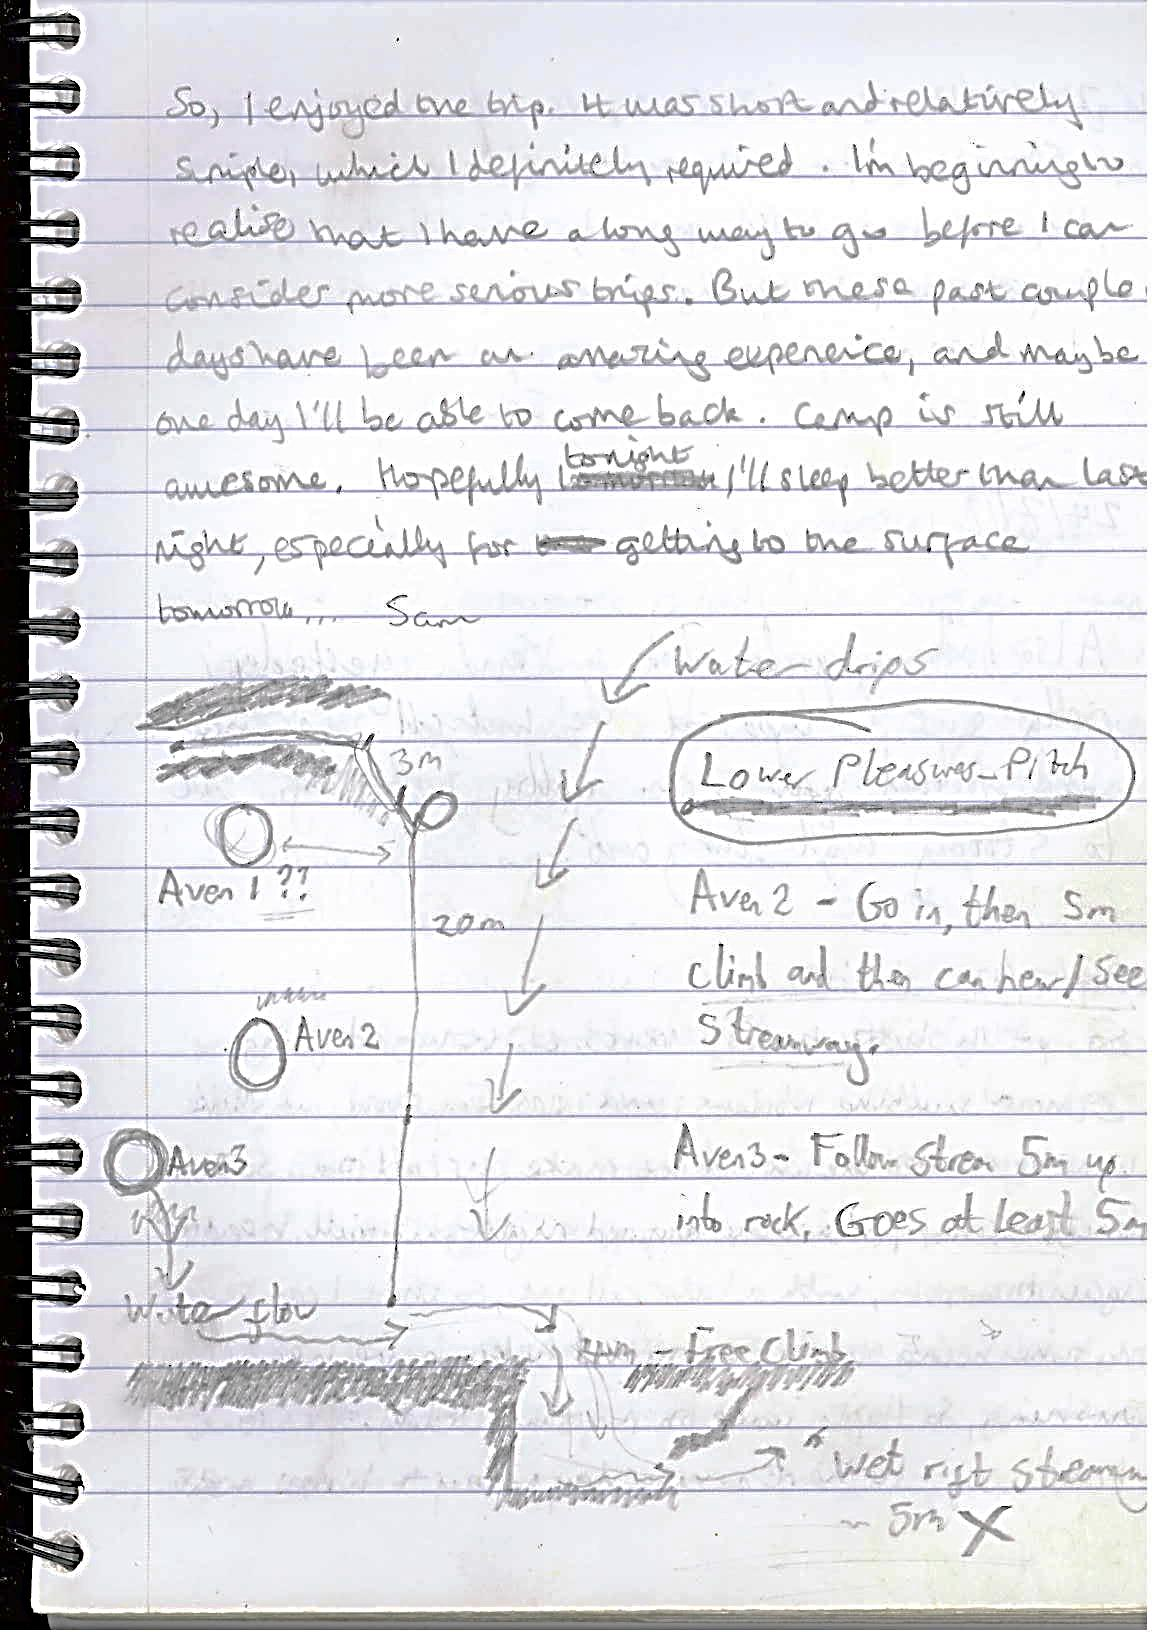
\includegraphics{appendices/ug_logbook/73.jpeg}\\
{[}Mike's sketch of leads at \emph{Lower Pleasures}{]}

\textbf{23/07/12 20:05 Sam}

Mike and I just got back from our trip. Although not particularly
successful, as the first trip of its kind for me it was hugely valuable.
We first headed off for \emph{Lower Pleasures}. Getting there was smooth
enough except a fair amount of time was spent removing a boulder from
one of the crawls. Once at the bottom, I poked my head around the
potential lead. Sloping up to the right was too tight; the only possible
way was ahead through a small rift with water at the bottom. (wet rift
streamway). Although I got a little way, the streamway narrowed so that
to continue one would have to be on their side, lying in water. Further
on, there was a very sharp corner which made it even more implausable to
try and pass. So, my first lead and a dead end! I then went up the first
rope and waited while Mike checked out another couple of leads, in a
couple of avens. Apparently these are promising leads, along with a
third aven which is harder to get to.

We then on our way back had a look around Xanadu. Nothing more was found
but it was fun to root around in such recently discovered passages. So,
I enjoyed the trip. It was short and relatively simple, which I
definitely required. I'm beginning to realise that I have a long way to
go before I can consider more serious trips. But these past couple of
days have been an amazing experience, and maybe one day I'll be able to
come back. Camp is still awesome. Hopefully tonight I'll sleep better
than last night, especially for getting to the surface tomorrow\ldots{}

\textbf{24/7/12 Sam}

Second night at underground camp was better\ldots{} I got a lot more
sleep. Looking forward to being back on the surface, despite feeling so
immensely confortable down here right now.

\textbf{24/7/12 Mike}

Also had a quick look in Xanadu yesterday; pretty sure I bypassed the
waterfall upstream and followed for 20 m getting wetter legs due to
stooping until turning back\ldots{}\ldots{}..

\textbf{24/7/12 13:00 Sam}

So, pretty shitty turn of events. I struggled going up \emph{Zimmer}
until the rebelays, and was very slow, and Mike was concerned we would
not make our call out. So I'm back in camp for another day and night,
and will head out again tomorrow, with a later call out, so that I can
take my time being slow. Jonny and Niko have headed out pushing, so I'm
in camp on my own today. It's the best way; to have an easy day today to
have max energy for tomorrow. My enthusiasm towards caving is at a
minimum right now. I would much rather be up top, but I'm ok lying
around down here. Hopefully when I am out, I'll be able to laugh about
all this, but right now I feel pretty damn awful.

\textbf{6ish Oli}

Camp X ray once again! It's far more pleasant than the surface has been.
Time for a quick smoke, piss, and 3 hours sleep to prepare for an
unexpected night train.

Niko comes back about 9:20 I haven't really slept much, but some nice
sugary tea is coursing through my veins

P.S. Thara snored for about an hour also, somehow, he managed to squeeze
in a sleep.

\textbf{24/7 Thara}

Nico: I don't want to see Gergely now. I'll be with another caver and
he'll be with another. It feels like cheating (on him.)

Oli: (answering the question of switching to night train) more caving
for the same amount of sleeping

Sam: When Oli and thara got here, I slept with them.

\textbf{24/7 22:40 Sam}

My afternoon was spent in camp, watching videos -- Withnail and I,
comedies, cartoons. I was pretty happy eating and watching. When Olli
and Thara arrived, I tried to get some sleep whilst they did; I reckon I
got about an hour and a half of sleep. Nico and Jonny back now, and
food.

\textbf{25/7 10:01 Oli}

Thara and I got back about 8:30, cooked some cous cous with large
quantities of ghee (someones genius addition to camp) resulted

{[}I CAN'T READ THIS SHIT.{]}

\textbf{25/7/12 830 Thara}

Back from \emph{Lower Pleasures}.

Still going horizontally if you are inclined towards Captain K.

Killed Sam's Aven 1,2,

Possible wet climb up Aven 3?

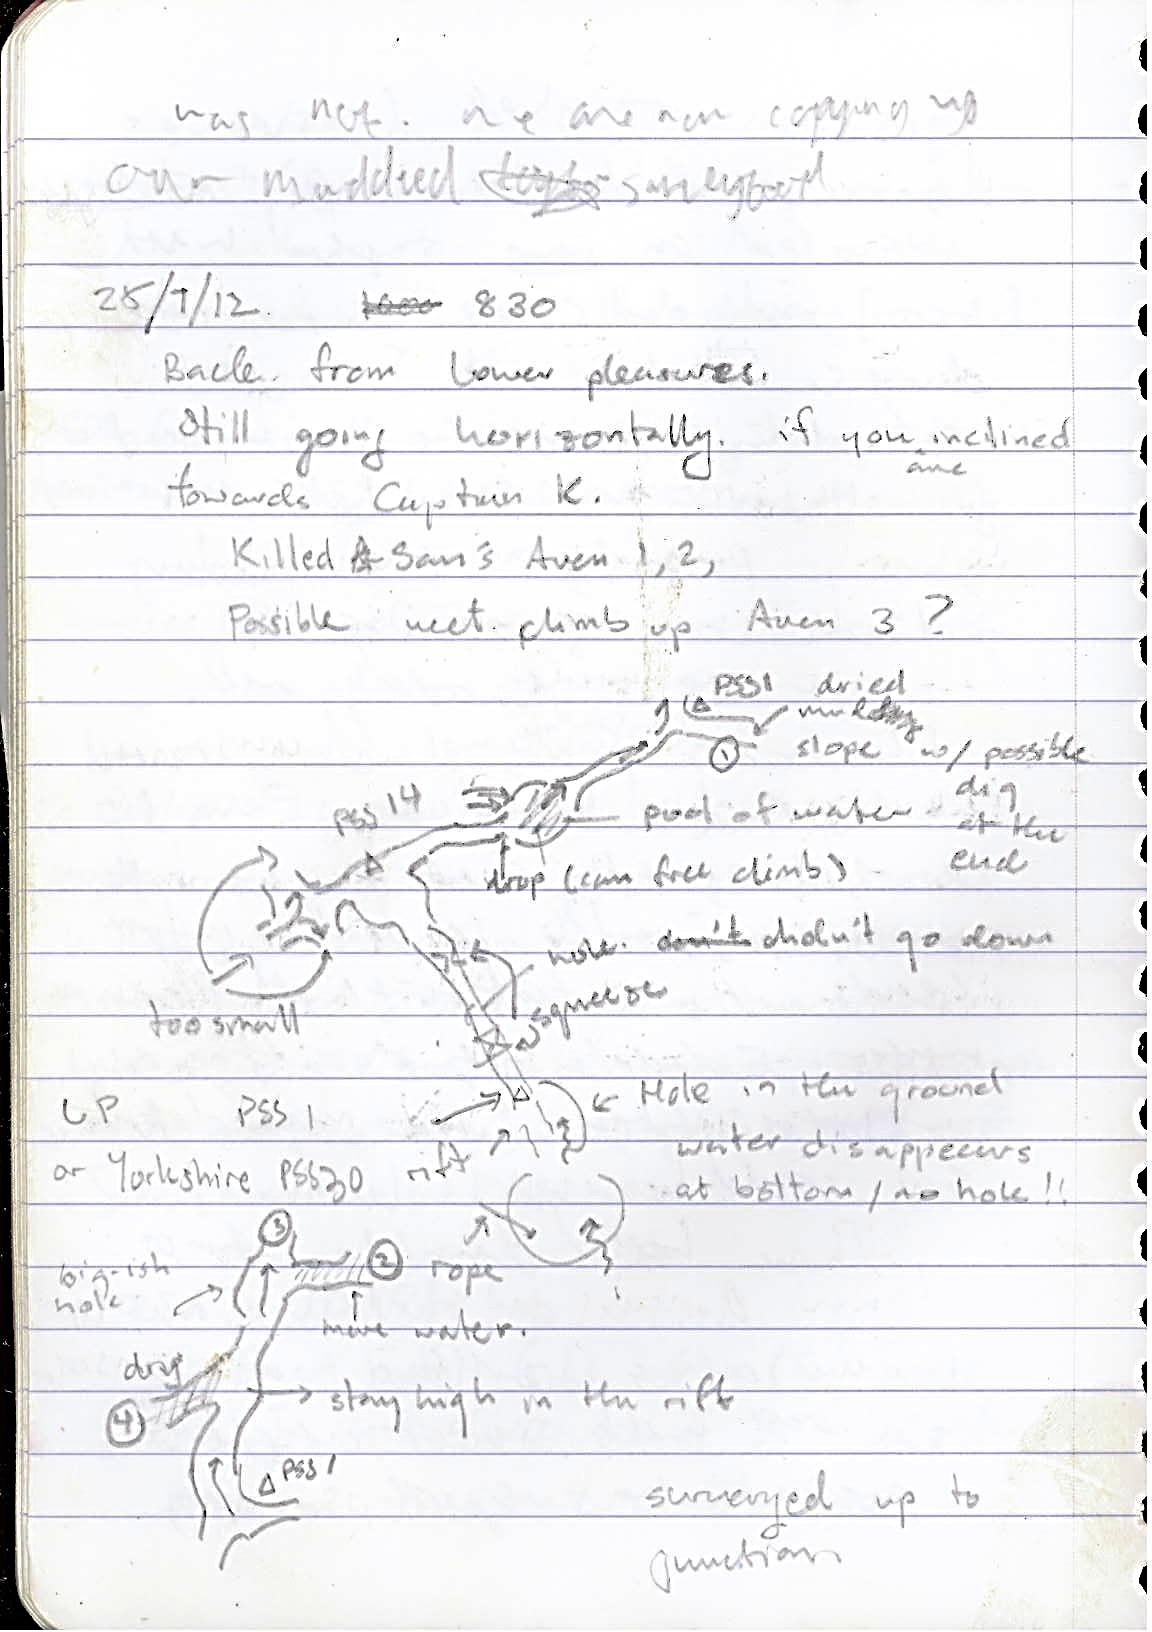
\includegraphics{appendices/ug_logbook/74.jpeg}\\
{[}Thara's sketch of \emph{Lower Pleasures}{]}

at the bottom it is like \emph{Yorkshire} cave!

\textbf{12:15 25/7/12 Jarv}

Here for a spot of Tea \& to escort Sam out. I've always wanted to run
an escort service.

\textbf{12:40 25/7/2012 Tetley}

Back again! Rhys and I got out fine 2 days ago -- we had 93 hrs
underground in all. Now here for daytripping, quick cup of tea and then
back up top with Jarv and Sam.

\textbf{11:24 Jonny 26/7/2012}

Woops, haven't written anything in the logbook yet\ldots{} Been down for
3 days and I've had a great time. Helped Sam out on our first pushing
day so had \textasciitilde 1/2 a day in the throne room, not too much
got done.

Went back yesterday and dropped 2 pitches to a boulder choke. Big wind
but it died at a dig

The lead at hot pants seems promising.

Overall, learnt a lot, had a good time and I feel I could stay down for
a few more days. To be honest, that probably would not be healthy.

The surface is calling!!

{[}Jonny's rigging guide for Why the Face?{]}

\textbf{26/7 12:20 Thara}

Oli + Thara went to Throne room / Hot pants to bolt climbing -- Epic
Fail!

\begin{enumerate}
\def\labelenumi{\arabic{enumi}.}
\item
  Our BDH for water leaked = only had 1 lt to share ½ of which was drunk
  without this knowledge (\textasciitilde 2:00)
\item
  Oli lost a spanner at Red Baron crawl (found later).
\end{enumerate}

-left at 12:30 after mega faff

Attempted bolt climb at the top at Hot Pants. Left for the next party.

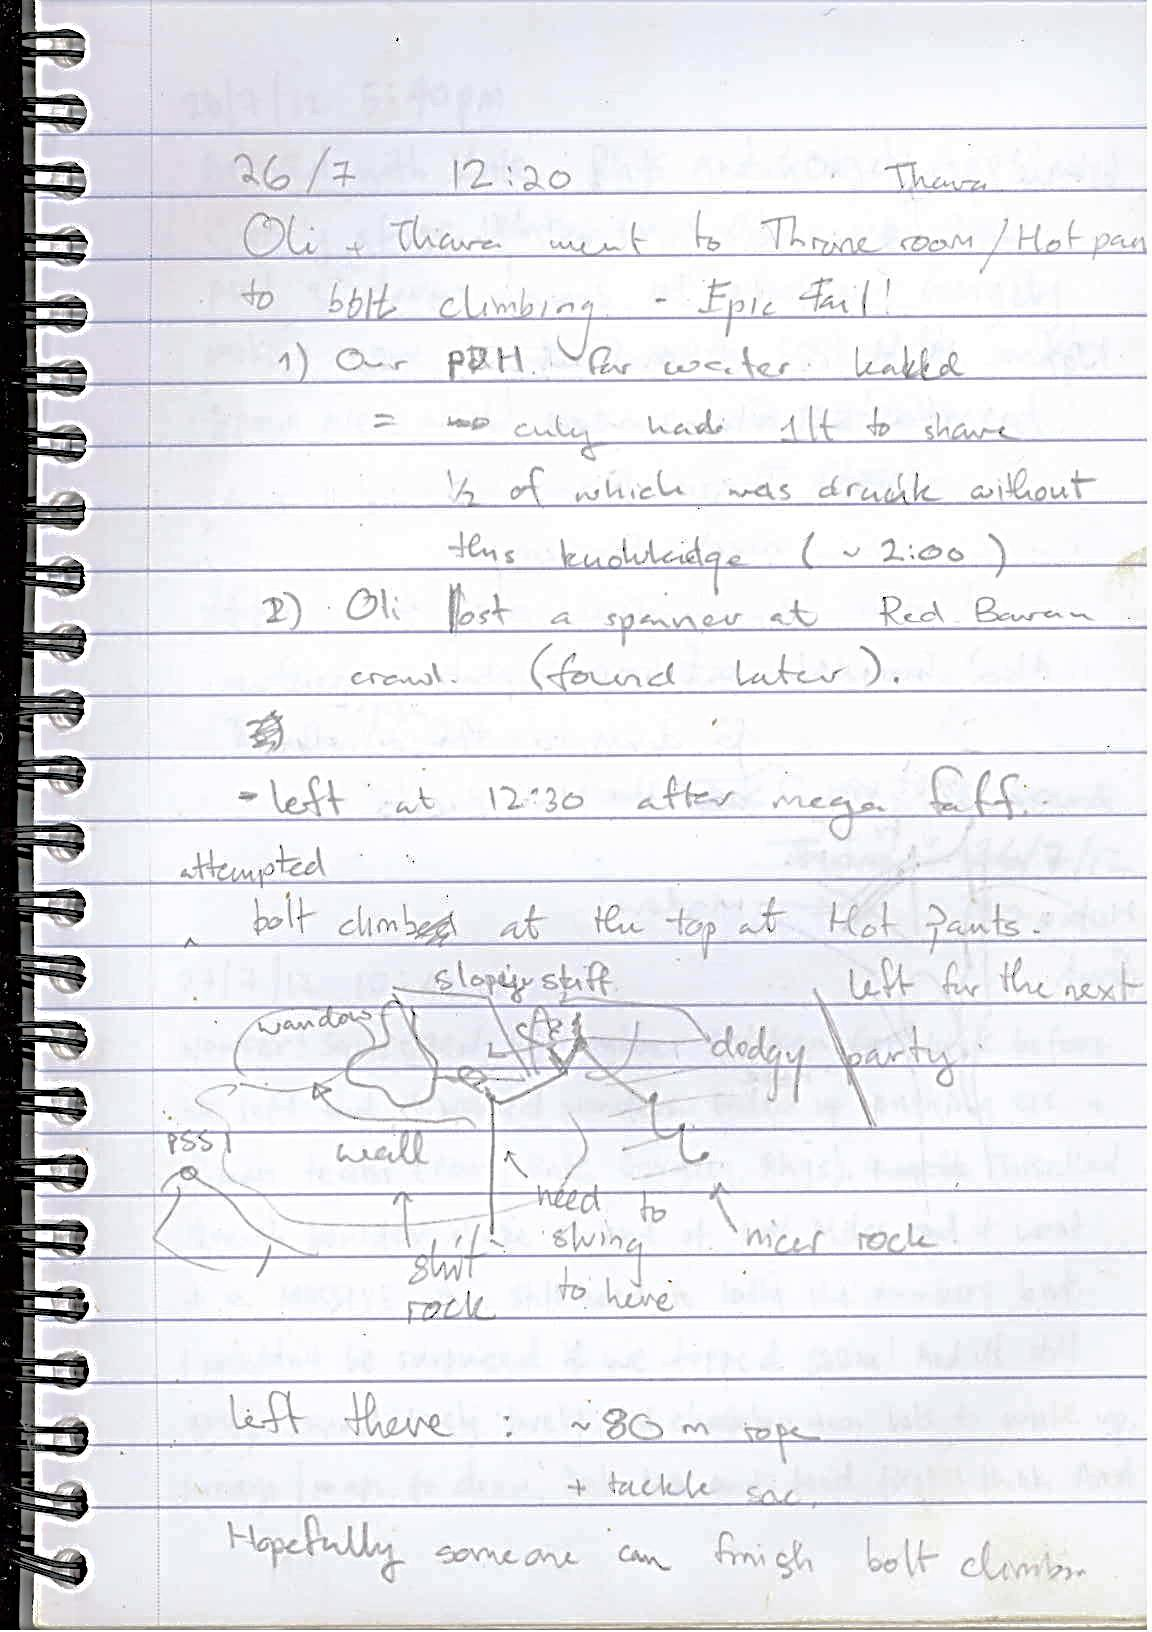
\includegraphics{appendices/ug_logbook/76.jpeg}\\
{[}Thara's rigging guide for Hot Pants bolt climb{]}

Left there: \textasciitilde 80 m rope + tackle sac

Hopefully someone can finish bolt climbs.

Back by 10:30

Possible name: Peep Show

Note: there is a lead in the floor near PSS Throne Room 5 need checking.

Also haven't set rope up to go down to the right window at Hot Pants.

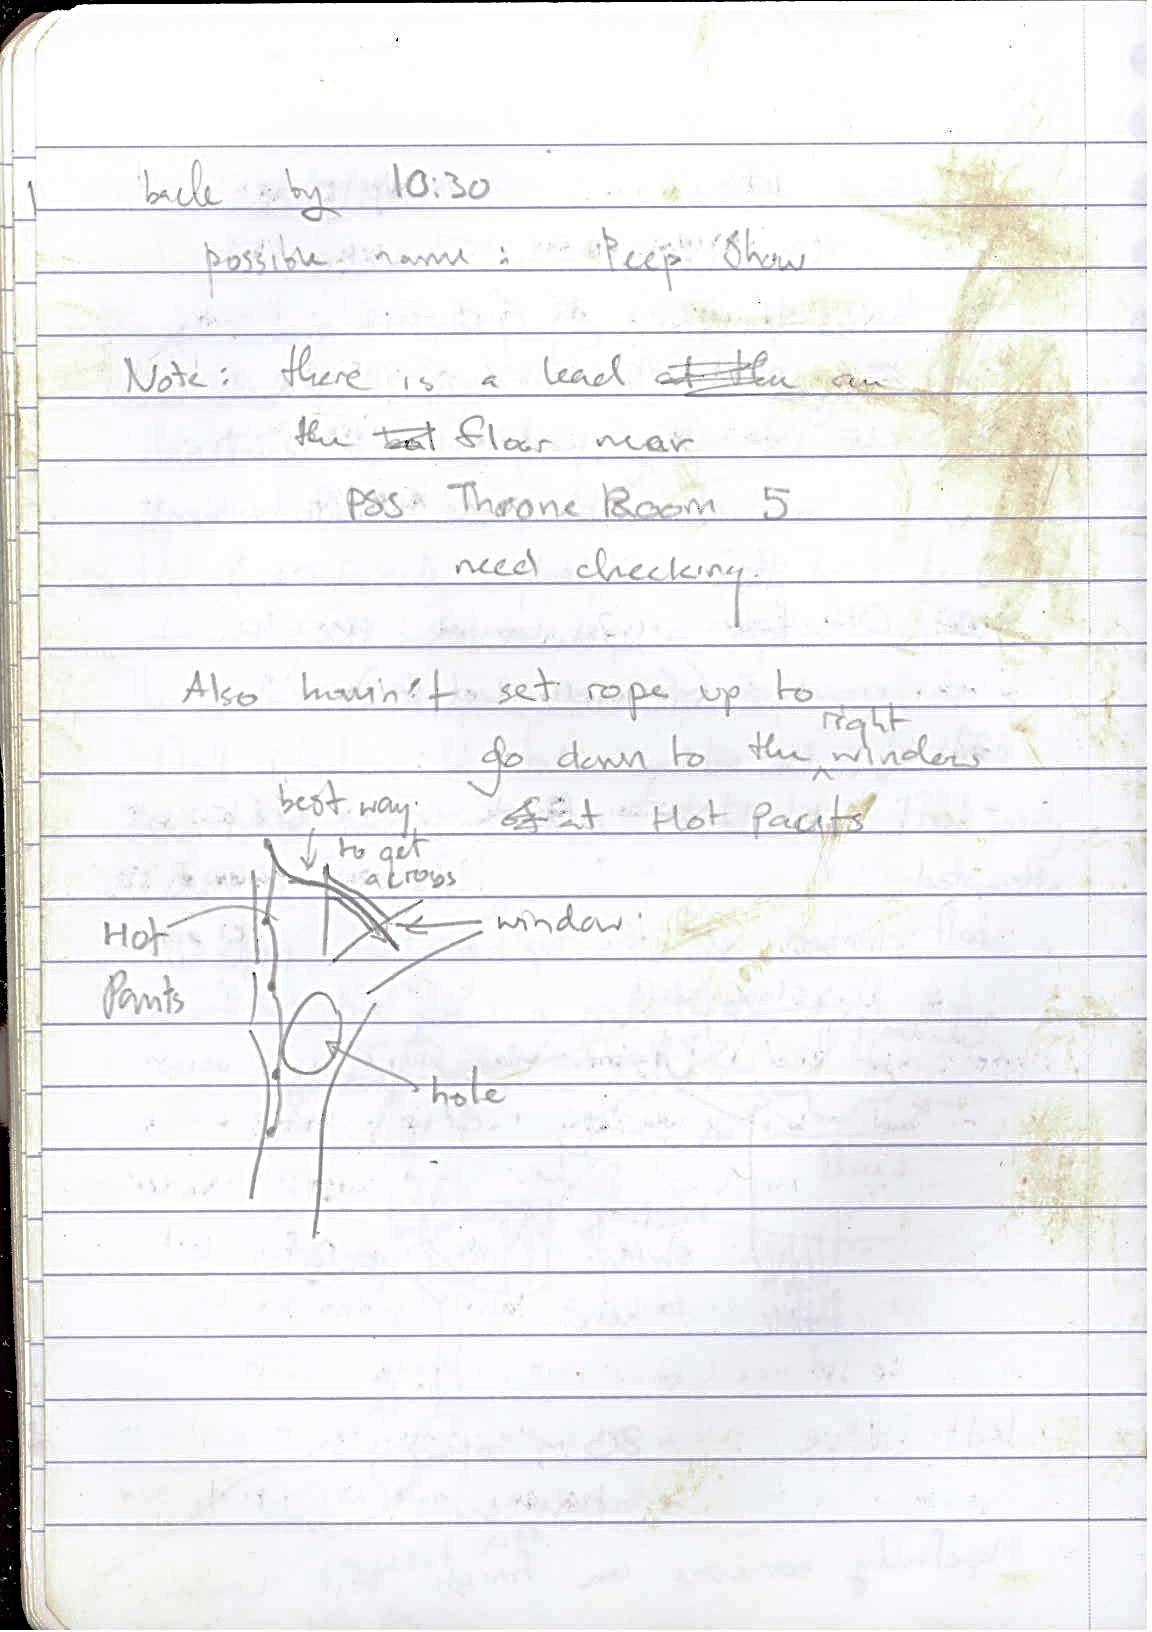
\includegraphics{appendices/ug_logbook/77.jpeg}

{[}Thara's sketch of Hot Pants window{]}

\textbf{26/7/12 5:40 pm Clare}

Arrived with Kate, Rhys and Gergely appeared shortly after. Water crisis
at camp! Just put 3 daren drums at \emph{Zimmer}. Gergely cooking now,
we will push Lost Miles and/or \emph{Brave New World} once we have eaten
meat.

\textbf{26/7/12 10 pm Thara}

After 54 hours underground time to surface and rise like a phoenix!
Thanks Oli. Good caving all round.

\textbf{27/7/12 10:42 AM Clare}

Wowser! Squeezed the rubber chicken for luck before we left and it
worked wonders. Ended up pushing as a 4 man team (Clare, Kate, Gergely,
Rhys). Chiselled through boulder choke at end of Lost Miles and it went
in a MASSIVE way. Still need to tally the numbers but I wouldn't be
surprised if we topped 500 m! And it's still going. Found lovely lovely
stal chamber too. Lots to write up, surveys/maps to draw, but tea and
food first I think. And sleep.

\textbf{7/28 6 am Gergely}

Yesterday pushed through the boulder choke we left w Izi last year, the
trick was to have a chisel w us. The passages down there seem to be
endless! Found about 650 m; mostly surveyed with the laser by Rhys \& me
(loads of 30 m legs). Still loads of leads (map to come).

Found water at the bottom of \emph{Stuck in Paradise} \& named that
chamber Hawaii -- a possible campsite. A bit epic trip of
\textasciitilde 21 hours.

Now off to Minotaur rift, checking out the squeeze at the end which
follows the fault line. Also changing some rope and checking the wind.

Good luck!

No music -- too bad.

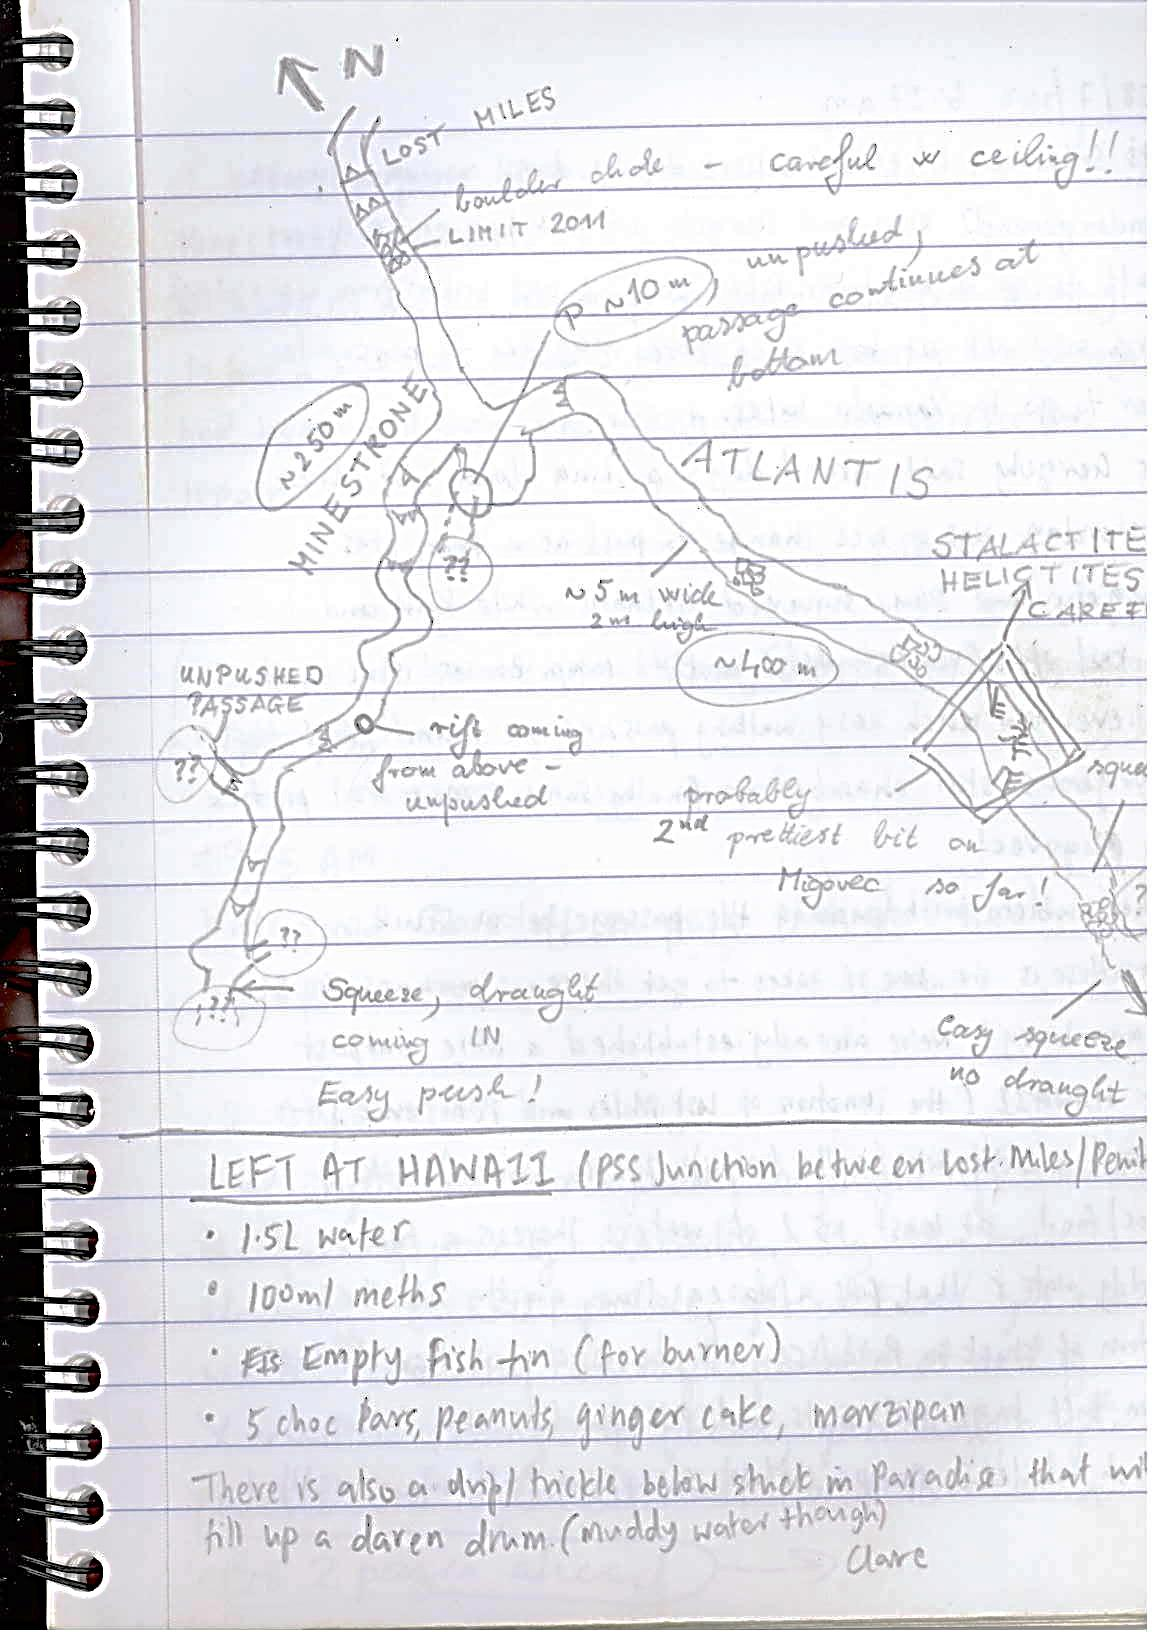
\includegraphics{appendices/ug_logbook/78.jpeg}\\
{[}Gergely's sketch survey of \emph{Atlantis} and \emph{Minestrone}{]}

\textbf{Clare}

LEFT AT HAWAII (PSS Junction between Lots Miles/\emph{Penitence})

\begin{itemize}
\item
  1.5 L water
\item
  100 ml meths
\item
  Empty fish tin (for burner)
\item
  5 choc bars, peanuts, ginger cake, marzipan
\end{itemize}

There is also a drip/trickle below \emph{Stuck in Paradise} that will
fill up a daren drum (muddy water though)

\textbf{28/7/2012 6:27 a.m. Clare}

It's Saturday already! Where do the days go when you're underground?
Rhys and Gergely are just beginning their faff to go to Minotaur Rift.
Kate is still broken from yesterday's trip so I will let her sleep more.
May try to persuade her to go to Xanadu later.

As Gergely said, grand day's pushing down Lost Miles yesterday. Was a
nice change to push as a four, plus Gergely and Rhys surveyed
\emph{Atlantis} while Kate and I fucked off (very slowly!) back to camp.
Bonus! Still can't believe how much easy walking passage we found. And
that gorgeous stal chamber -- finally some proper stal pretties on
Migovec!

The problem with pushing the passage below \emph{Stuck in Paradise} is
the time it takes to get here\ldots{} perhaps a little 2 man bivvy?
We've already established a little outpost at HAWAII (the junction of
Lost Miles and \emph{Penitence}) -- there's a brew kit (meths (100 ml),
fish tin burner), bits of choc/food, at least 1.5l of water. There is a
trickle of muddy water that fills a daren drum quickly at the bottom of
\emph{Stuck in Paradise}. Maybe a 4 man team to bring down buff bags,
roll mats and pots, candles etc, then 2 push while 2 sleep, before
swapping? Hmm\ldots{} well, I know I'm going back to \emph{Brave New
World}/\emph{Atlantis}/\emph{Minestrone} regardless!

We have no music at camp -- came back from pushing to find a note from
Thara + Oli saying the charger had broken and they were taking it to the
surface for repairs.

(Rhys + Gergely callout 8pm, expect to be back 4 or 5 pm)

\textbf{9:15 AM Clare}

Kate and Clare off to push Xanadu. Back by 4pm.

\textbf{2:00 pm Kate}

After some route finding in jungle rift found the pushing front of
Xanadu. By this time already I had foolishly got wet and got even wetter
crawling through puddle at end of Xanadu. Passage quickly gets bigger
after puddle and after a small climb there is a pitch left unrigged that
can be pushed. We started surveying the \textasciitilde 30 m of new
passage but before we could connect to Xanadu got too cold and
instruments too muddy to carry on. Only 2-3 legs to connect but
unfortunately there will be a station in the puddle. V. cold still so
writing illegible \& unintelligible. Defo learnt my lesson though. Don't
get wet whilst pushing! Xanadu is cool though, you should go.

\textbf{28/7/12 2:10 pm Clare}

Kate and I went to Xanadu for some easy pushing. Named our finds
EUPHRATES. It is possible to not get too wet crawling through the
puddle. Unfortunately what was nice dryish sandy passage after the
puddle is now a muddy crawl!

* EUPHRATES PSS 11 and Xanadu PSS 18 need to be tied in. It is only 3
survey legs. Kate got hypothermic and instruments got too muddy too read
so we turned back. At the end of Euphrates is a 5-10 m pitch,
draughting. Bring rope!

Will try to sleep now in case a day train arrives to kick us out of bed.

\textbf{28/7/2012 9:20 pm Gergely}

Just got back \& had dinner \& tea \& Vitaminski with Žganje, which is
great.

Today we pushed the squeeze at the far end of Minotaur rift. It was
pushed by JKP to a boulder choke before. The place is interesting
because it directly follows the fault line of Minotaur rift. So we
headed there with Rhys. On the way there, we rerigged the handline to
Leopard, the top rebelays of \emph{Cheetah}, and the traverse in Prince
Consort road. And had a look at Queen's Bedchamber -- the climb seems to
be doable!

So, the crawling passage goes. But not easily. The passage is usually
0,5-1 m high, 1 m wide, full of sharp rocks, and both the ceiling and
the side walls tend to fall off. We got through the first boulder choke
in about 2 hours. Then, immediately after, found a squeeze with 3 large
boulders, which we couldn't remove. Luckily, there is just enough space
to squeeze through (but it is tight for us as well!)

The third choke gave the name to the passage. So there the continuation
goes down on the left. However, large bits of rock are on top. A fat
rock of size \textasciitilde 1.5 m x 1 m was just in front of the
passage, but when we tried to move it, it started to slide down \&
almost blocked the continuation. We managed to stabilise it somewhat,
but as you go down, your head is just below it\ldots{} Good luck! So,
the name is GUILLOTINE.

Altogether, we found about 85 m of squeezing passage. Then, first we
found a small chamber off to the right with water, and the fault line
\textasciitilde 10 m long, \textasciitilde 5 m high. The stream goes off
to a tight meander. Continuing in Guillotine, a further 30 m brings you
to an opening to the right -- and you find yourself at the top of a
\textasciitilde 30 m high rift! This is along the same fault line as
Minotaur, but is an active streamway. -- we could hear water at the
bottom. It is large, and goes directly towards the System. Beautiful
white walls!

In the squeeze, we found hematite pebbles and sometimes along the fault
line, the rock looks like marble, which would be very nice apart from
the fact that it constantly falls on your head.

So, altogether, we are \textasciitilde 100 m closer to the System on
this level, and the continuation is at the bottom of a large, open rift
-- sounds quite good\ldots{}

Now, time to sleep and hope nobody comes.. We managed to shift back to
the day train. Good luck.

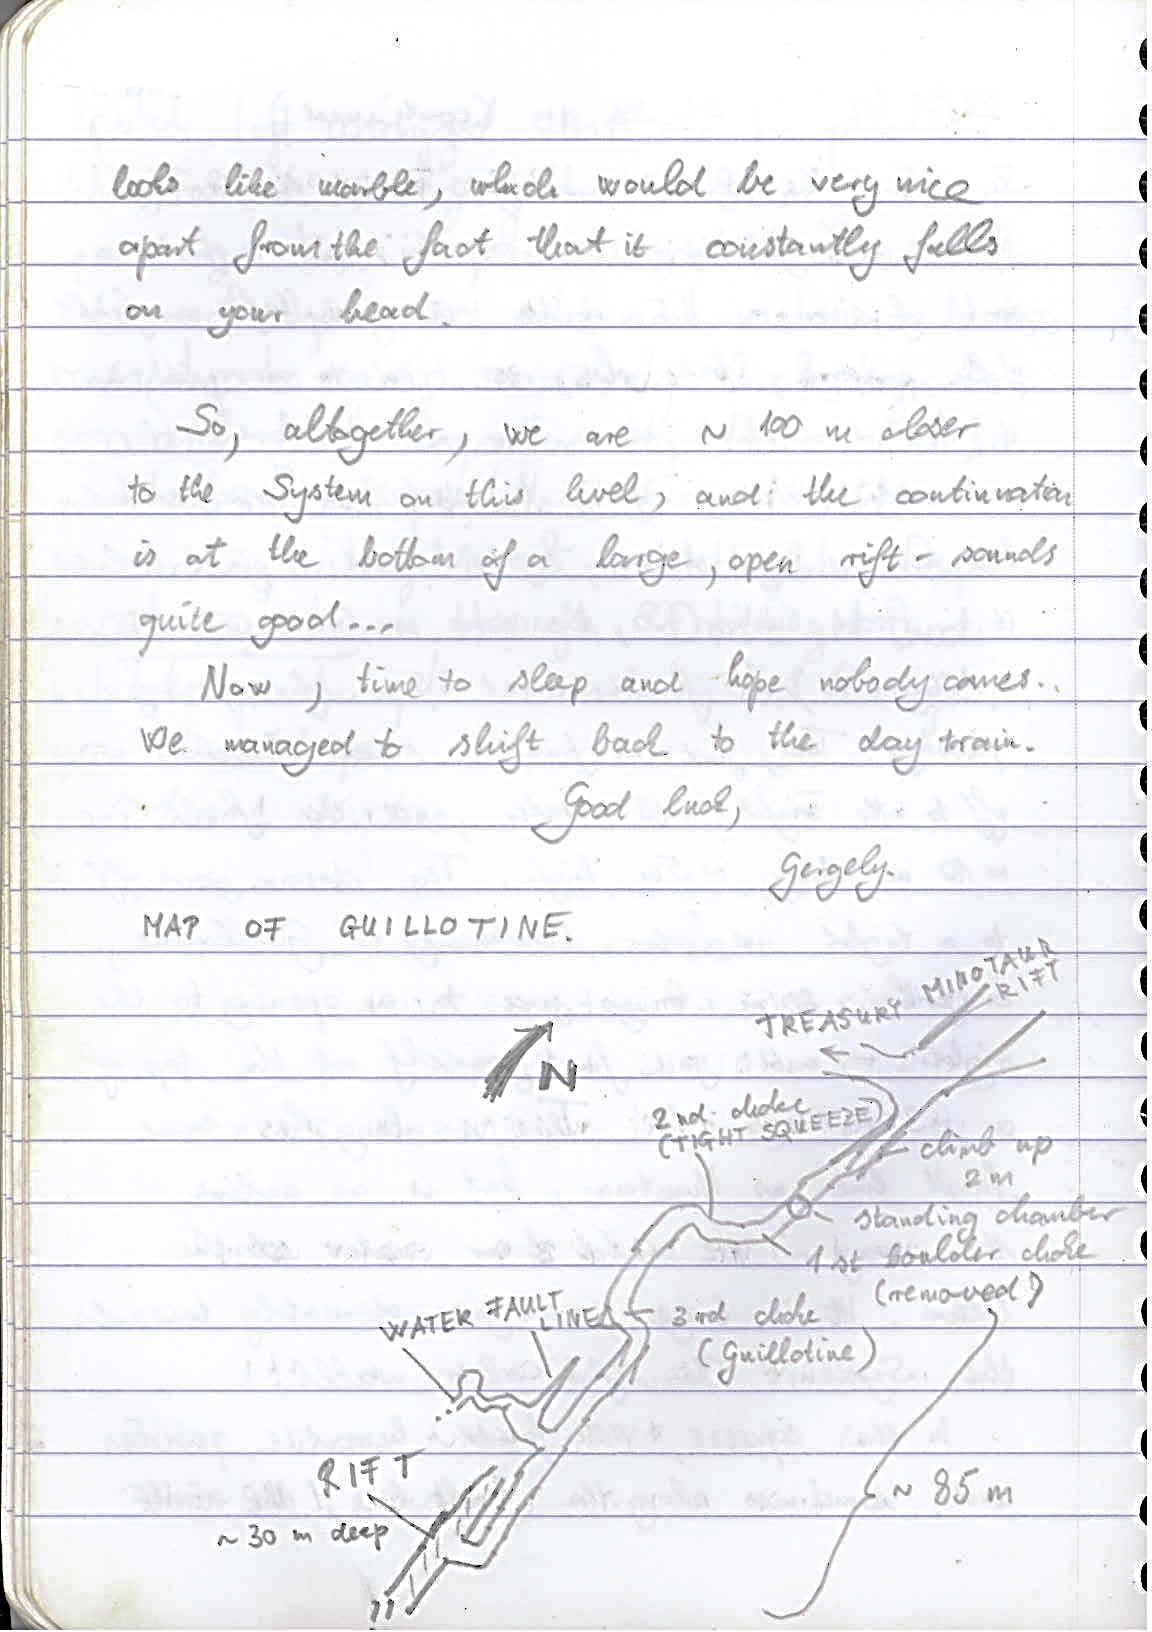
\includegraphics{appendices/ug_logbook/79.jpeg}\\
{[}Gergely's map of Guillotine{]}

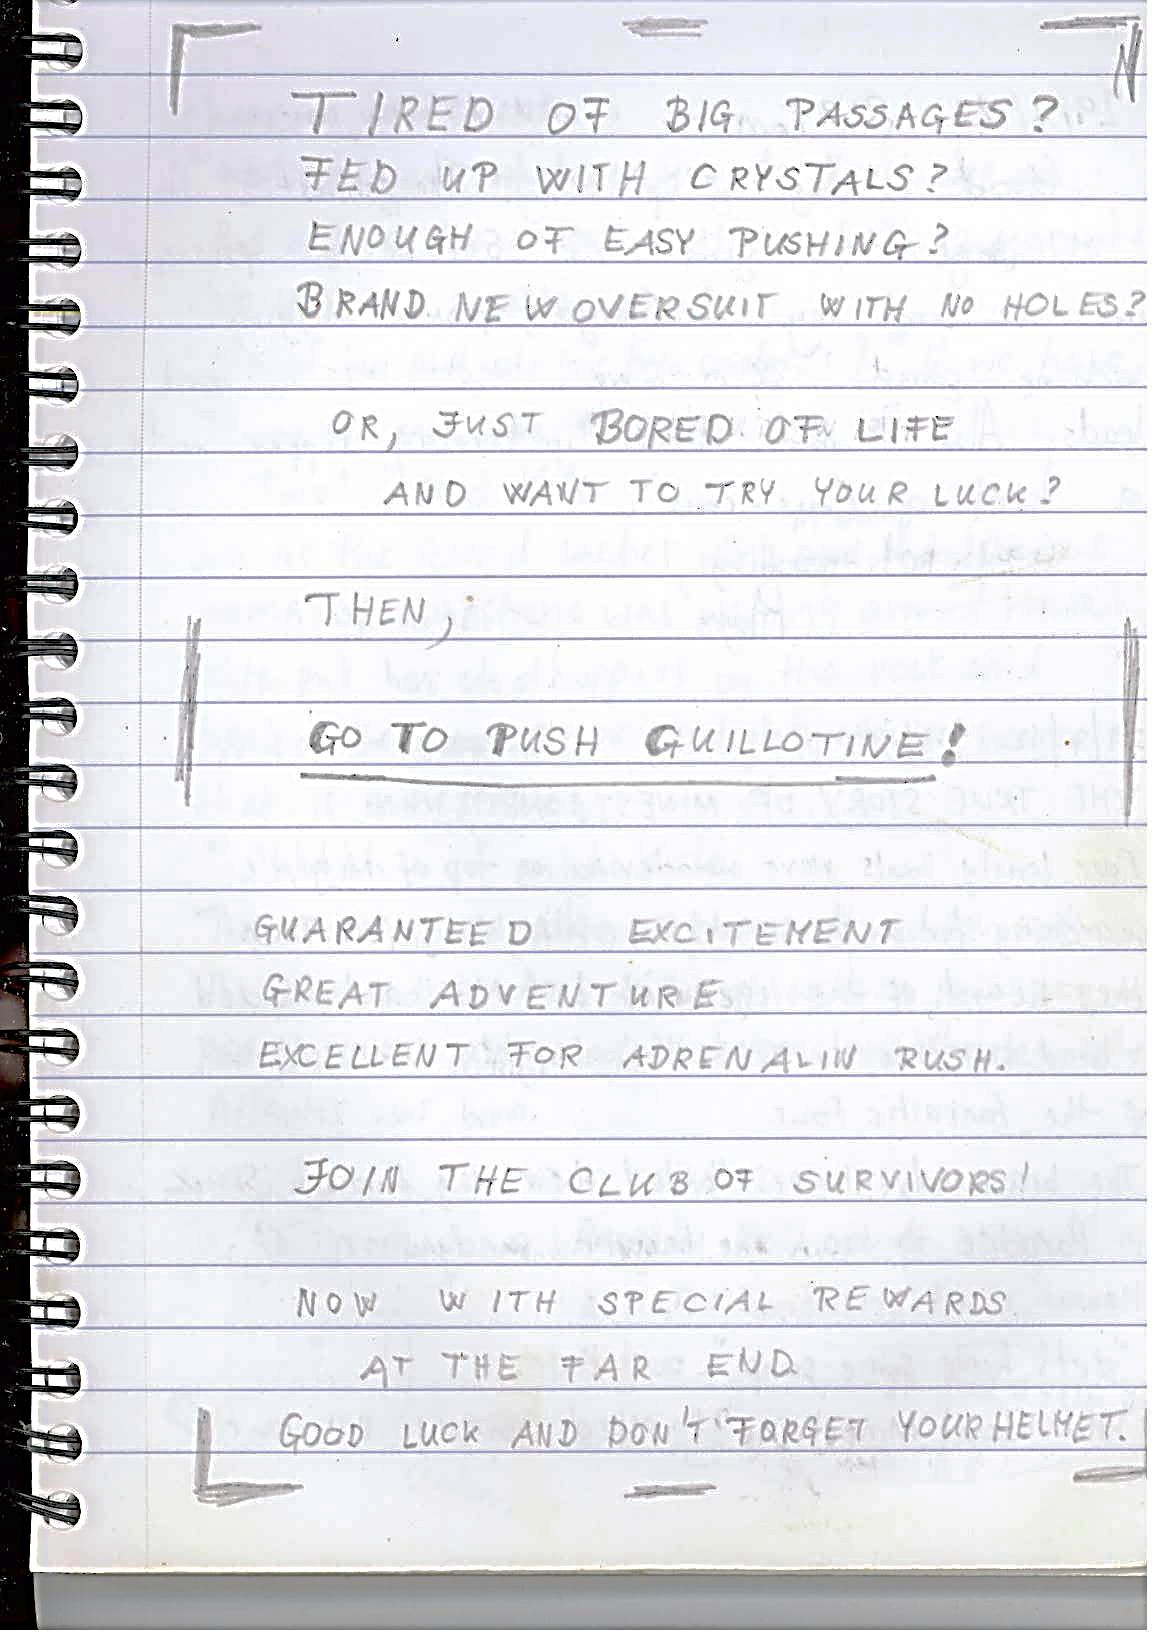
\includegraphics{appendices/ug_logbook/80.jpeg}\\
{[}Gergely's recruiting pitch for Guillotine{]}

\textbf{29/7/12 8:27 am Rhys}

Good 2 days of pushing. The fantastic 4 managed to find over 600 m of
passage and me and my 1 Gergely-power digging machine found 80 m more!
Left lots of good leads. Also I made dinner yesterday `Pepper with a
hint of Cous-cous!

Good luck pushing.

\textbf{29/7/12 9:36} \textbf{am} \textbf{Gergely, Kate, Rhys, Clare AKA
The Fantastic Four}

THE TRUE STORY OF \emph{Minestrone}

Four lonely souls were wandering on top of Migovec searching for a cause
worthy of fighting for. Then they heard of the legend of Lost Miles and
decided to band together to create the almighty caving force of the
Fantastic Four.

The brave adventurers battled their way through \emph{Stuck in Paradise}
to reach the beautiful sandy shores of Hawaii.

``Let's have some soup,'' said Kate.

``How about \emph{Minestrone}?'' asked Gergely. All four cheer in
excitement.

``Now guys, whatever you do, don't step on this rock or the
\emph{Minestrone} will go everywhere,'' Kate said in a superior air.

``Should we put one or two sachets? If we have one we can save the other
for later.''

``Two!'' said Kate.

Just as the second sachet went in and the delicious aroma of
\emph{Minestrone} was wafting around Hawaii, Kate put her clodhoppers on
the rock and toppled the almighty power source that is
\emph{Minestrone}.

``Ohhhhh\ldots{}'' said Kate.

The rivers of spilt \emph{Minestrone} flowed towards the promised land
of 650 m of walking passage. And thus the passages of \emph{Minestrone}
and the beautiful \emph{Atlantis} was born.

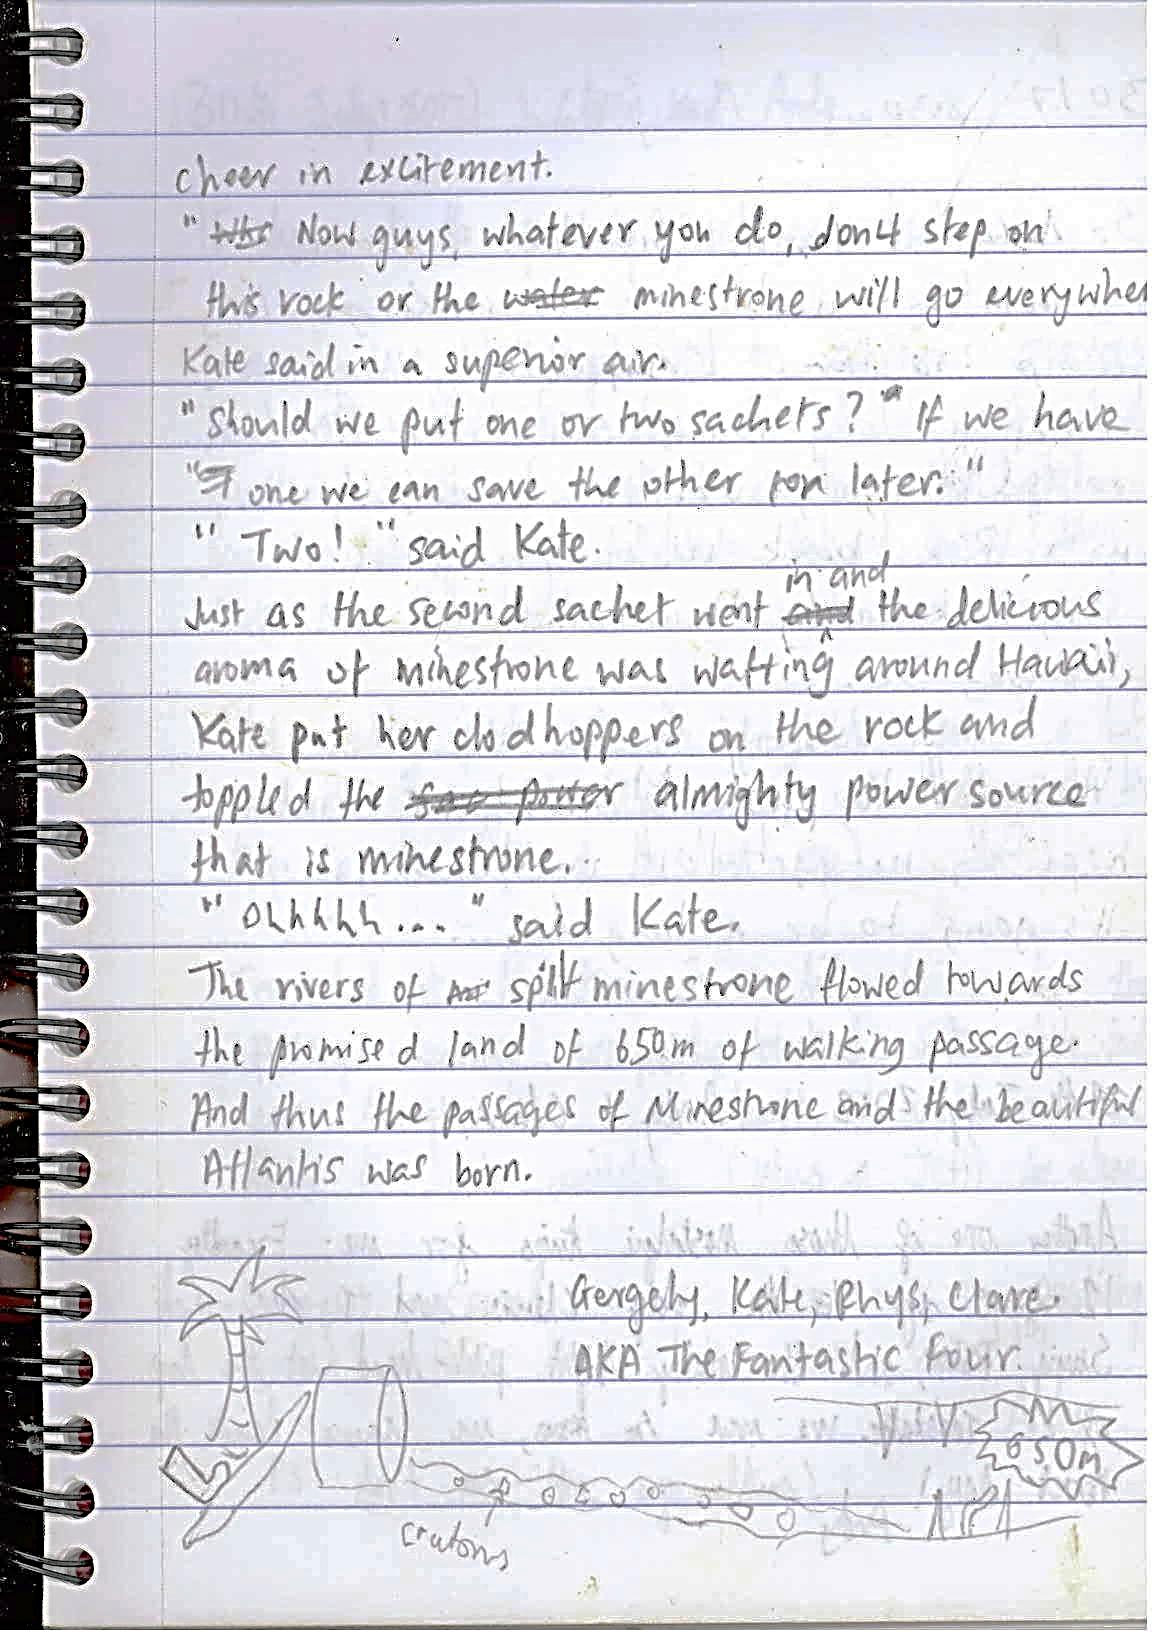
\includegraphics{appendices/ug_logbook/81.jpeg}\\
{[}Kate's illustration for The True Story of \emph{Minestrone}{]}

\textbf{30/7 8:30 am Clewin}

Andy Jurd \& Clewin Griffith

So Andy and I just finished probably my comfiest night at an underground
camp so far. Camp \emph{X-Ray} has come a long way since the first cold
\& draughty version I stayed in with Rik back when we pushed Big Rock
Candy Mountain and Highway 32.

We're off to push \emph{Minestrone} and hopefully not get lost on the
way. It's going to be a long day\ldots{}

\textbf{29\textsuperscript{th}} \textbf{July 2012 -- Andy}

Andy + Clewin

Another one of those nostalgic trips for me: Exactly 12 years ago to the
day Clewin and I discovered Swing Pitch, and the really tight pitch-head
at the top of the Tessolater. We were so keen, we came back the next
day!

\textbf{30\textsuperscript{th}} \textbf{July 2012 -- Andy}

Clewin and Andy

15 hours to the pushing front and back\ldots{}

Even if we didn't get lost on numerous occasions, there still wouldn't
have been time to do any actual pushing! What a waste of a trip -- but
good exercise taking rope/drill/electric bits and bobs/survey stuff
there and back!

That muddy pitch with the forgettable name is a bit rubbish too -- yuk!
(there is a water bottle under the drip to the left of the last rope).

The lead at \emph{Minestrone} is a bit rubbish too -- the passage
becomes completely blocked with rubble, but even though there is a
draft, it would need more than the two available (plus a JCB) to clear
it!

Suggest a second camp closer to the pushing front! -- But there's not
much water!!!

PS don't use the eye-lotion!

PPS -- too cold for the class to work -- suggest taking the cylinder to
bed with you!

\textbf{Jarv 31-7-12 3:51 PM}

Dropping by on a solo bounce.

I deliver: 1 fin

1 faber 7L 232

w/ 220 bar air

8 kg lead on a belt

Trying to squeeze 1 lukewarm coffee out of the gas canister -- gobble a
few midgets \& then depart for the surface.

Mmm, gas died -- onto the meths!

Interesting trip down -- rope work was OK but arduous.

Freeclimbs were scary -- 20 kg of extra weight made stepping down to a
foothold v. dodge!

Camp seems nice -- a pity to see it so empty though ---

So:

\textbf{1/8 /2012 JONNNY (+ NICO) 19:00}

Ahhhh!! Back in camp!

Hand a morning/afternoon working super-hard in the bivi (ahem\ldots{})
and a faultering of enthusiasm when entering the cave. As such, our
pushing for today shall be limited to pushing play on the music player.

Checked that the drill is ready for a trip to Throne Room tomorrow and
it all appears to be in shape

OH NO, can't get music player to work

Nico:

``I stopped listening for 3 seconds because I was desperately trying to
get my cock out''

\textbf{2/8/12 Izi}

Mawer in Izi

Prvo sva splezala enih šm v Minotaur Rift, gre še naprej, samo je plast
zemlje enih km na dolyem, ki je nisva vspela preplezat. Pol sva šla v
Queen bed chamber, tam sva splezala 6 m višje od lani, že zmer je do
vrha enih 6 m + je treha traverzo da prides do dobre skale.

\textbf{2/8/12 JANA}

JANA and GERGELY

GUILLOTINE -\textgreater{} RAZOR

Amazing to follow the fault line in such way, so close. Very tight in
places. Surveyed about 60 m. From Guillotine passage you pop out in open
space, called Razor. ``Dead'' as to tight to follow the crack,
possibility to climb up (\textasciitilde 20 m) look like could be a
higher passage. Way back was shitty, dragging 2 bags up 100 m tight
slope.

Time to rest now.

\textbf{Jarv -- 2/8/12}

Frustrating time down `Esoterica' -- if that is where we were.

I think that Jan \& James traversed over the pitch we wer trying to get
down. We failed -- driver broke.

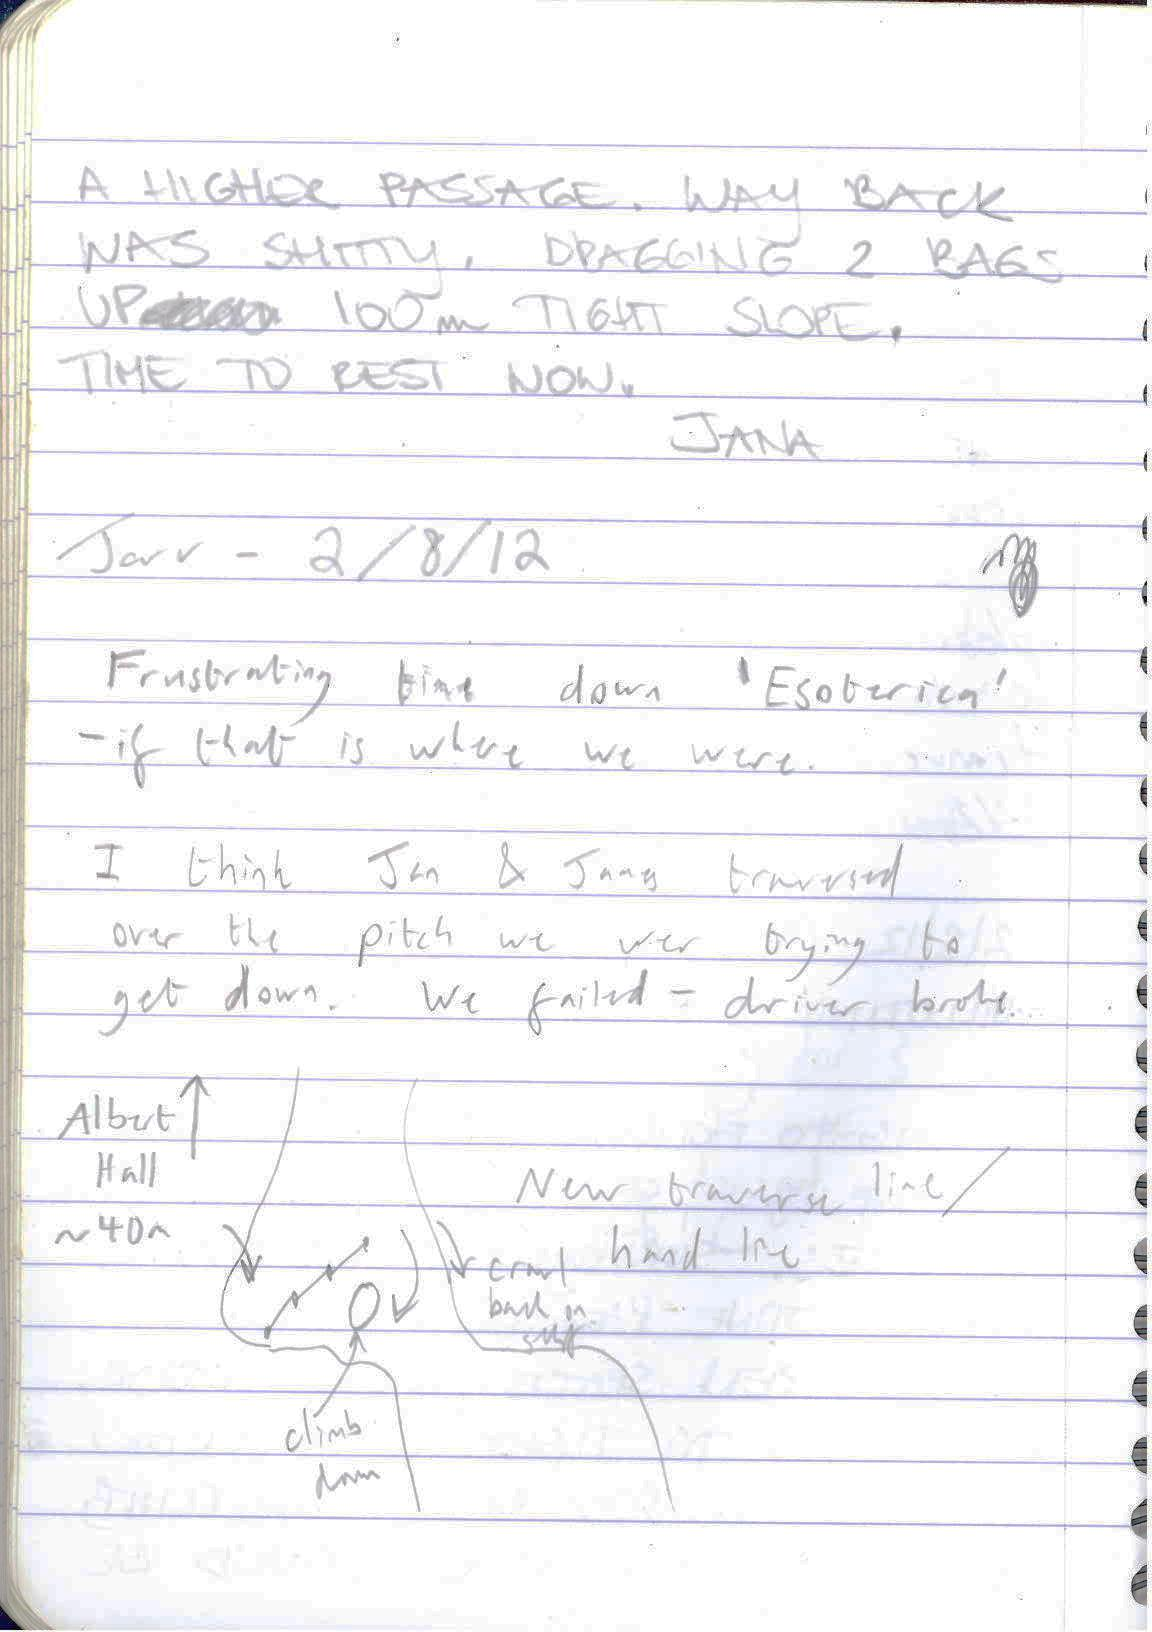
\includegraphics{appendices/ug_logbook/82.jpeg}\\
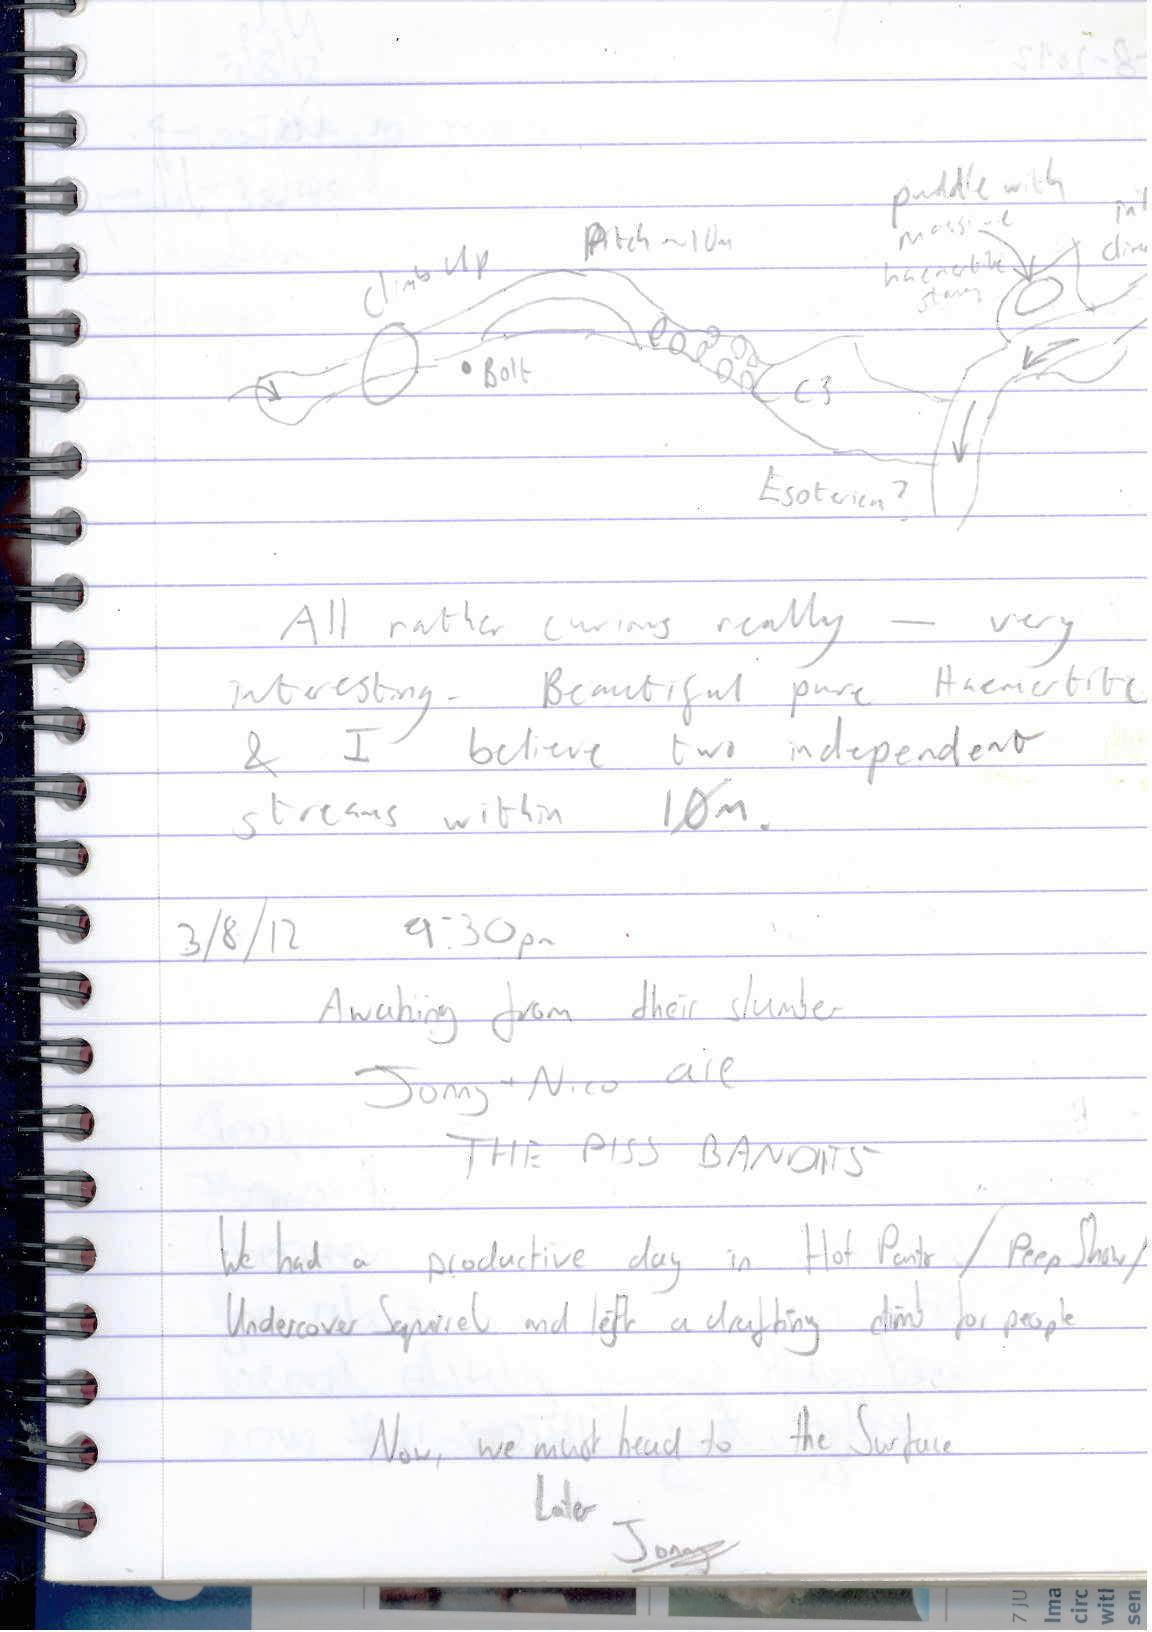
\includegraphics{appendices/ug_logbook/83.jpeg}\\
{[}Jarv's sketch of Esoterica{]}

All rather curious really -- very interesting. Beautiful pure Haemertite
\& I believe two independent streams within 10 m.

\textbf{3/8/12 9:30 pm} \textbf{Jonny}

Awaking form their slumber.

Jonny + Nico are

THE PISS BANDITS.

We had a productive day in Hot Pants / Peep Show / Undercover Squirrel
and left a drafting climb for people.

Now we must head to the Surface.

\textbf{3-8-2012 Niko}

Alrite wackos, my last morning in UG camp. Quite a trip. Doing these
couple of pushes Johnny \& me formed this deadly \& amazing combo ``the
Piss Bandits!''. Overall we found 3 passage thingies ``Why the Face?''
``Peep show'' ``Undercover squirrell''. Loadsa fun, glad I was part of
it this year. Rock on UG camp, Sayonara from Niko

\textbf{3-8-12 Jarv}

Another glorious morning at Camp \emph{X-Ray} -- this one actually a
morning. Bowie on the fixed stereo. Our plan: Watership Down, below
\emph{Daydreamers}/\emph{Insomnia}/\emph{Republika}/Mad Cow. A long way
down -- to -900 m.

\begin{itemize}
\item
  Be very careful with the AA-\textgreater{}MP3 lead -- just charge the
  player \& then put it somewhere safe
\item
  Don't use comf for a pillow -- it get soaks with condensation!
\end{itemize}

\textbf{3/8/12 Jana}

JANA, IZI, MAWR, GERGELY = The Eastern EU team

WENT TOGETHER TO HAWAII CAMP, WHERE WE SPLIT IN 2 TEAMS:

GA + NM -\textgreater{} \emph{Brave New World}

JC + IM -\textgreater{} \emph{Atlantis}

JANA and IZI

We have not seen the new stals etc, so we went to have a look + to take
some photos. Acording to Gergely the way on was ? and tight. We found 2
ways on we chose the Right one as it looked less tight. After a squeeze
we went down a small dry muddy sloape popping into very small
``chamber''. From here a super tight squeeze (between rocky celing and
floor) for about 10 m. A water was heard already from the beginning now
the noise just getting louder. We came out like at the bottom side of a
very big pitch above. A new big waterfall coming down and a good amount
of water going down. We free-climbed down to the bottom of it. Got wet
under the waterfall. Very big place, looks like a canyon, we continue
climbing down, following watter and eventually stop as rope is needed 2
get down. As far as Izi could see there were water pools.

Very interesting finding after so many dry passages.

A place where we need to go back!

We named it: BREZNO SLAPOV -\textgreater{} Waterfall Pitch

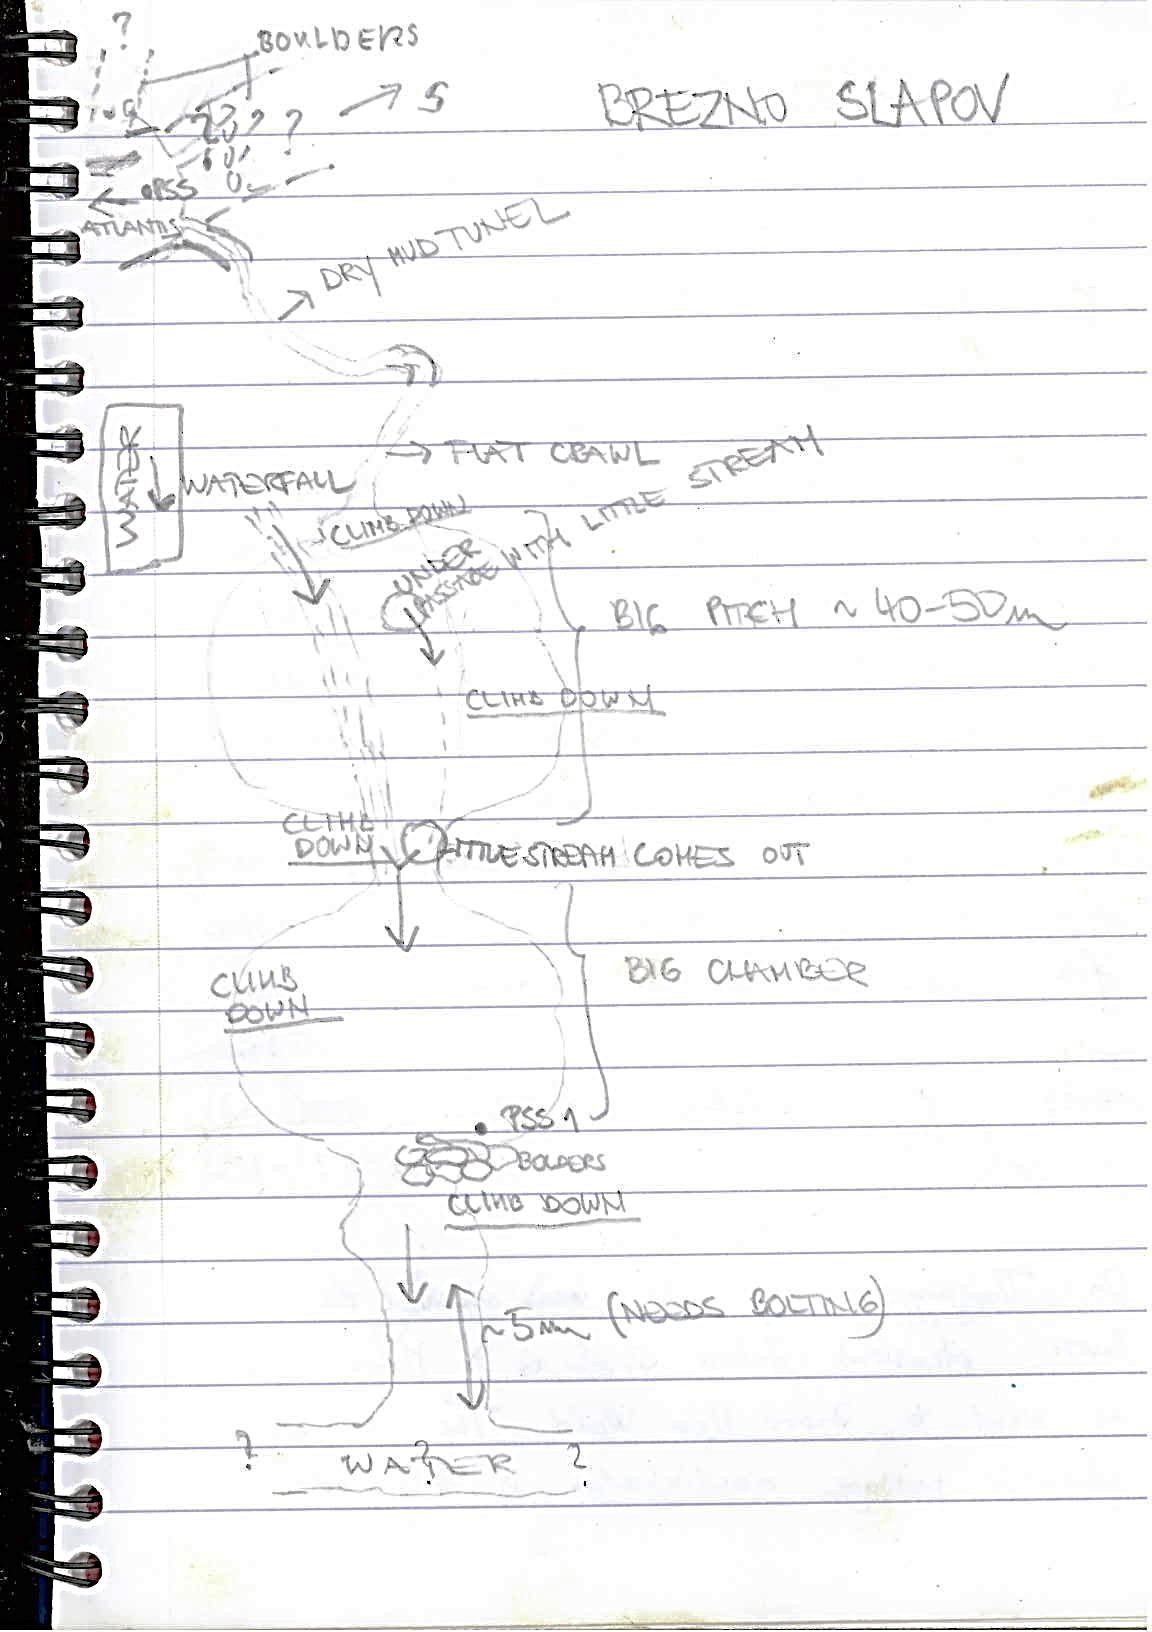
\includegraphics{appendices/ug_logbook/84.jpeg}\\
{[}Jana's sketch of Brezno Slapov{]}

\textbf{3 August 11.30 am Gergely}

Once again, in camp, with `Team Eastern Europe'! the first day, we went
to Minotaur Rift. Izi + Zejc climbed the window on the right and then
continued the climb in Queen's Bedchamber; both projects are to be
finished. Jana and me went to Guillotine to rig the rift at the end. We
managed to get there with the 2 tacklesacks and rigged the pitch, but it
dies at the bottom. However, above us in the \textasciitilde 10 m height
a wider space is visible. The rift is \textasciitilde 30 m high. You can
also see a window of the continuing rift towards South. Another
possibility would be to gain the height at the beginning of the crawl;
one can see \textasciitilde 15 m up here.

{[}Gergely's sketch of Guillotine{]}

On Thursday/Friday night, we checked the lower extensions below Stuck in
P. Mawer and me went to \emph{Brave New World}. The obvious phreatic
passage continuation is blocked badly by collapsed ceiling (massive
boulders). Possible way should be towards the left, but we did not
manage to get through. It will be hard work. Strangely, we think that
the draught going out there is less than before. Part of it also goes up
in the rift/stream on the left, that we climbed \textasciitilde 10 m,
but it gets too small after a small pool. We also tried to find a bypass
to no avail. I think that the eastern front will be hard to push.

On the other hand, Jana + Izi's find is super interesting. The main S
passage (\emph{Atlantis}) continues the same direction; I checked the
pitch at \emph{Atlantis} \& \emph{Minestrone} (free climbable) and the
passage goes at the bottom! Plus the unwalked passage off
\emph{Minestrone}. Great leads there! The southern front goes goes goes!

Good luck.

\textbf{3/8/2012 15:00 Tetley}

Back here with Rhys after 4 days of holiday in London! We're off now to
look at \emph{Brave New World}, may then check out other leads below
Stuck in Paradise.

We'll leave note(s) to say where we are! Back here by 11am (4/8/12) at
the latest!

\textbf{3/8/12 18:00 Dan}

DAVE +DAN off to \emph{Big Rock Candy Mountain}. Back approx 20-00

\textbf{4/8/12 1100 Izi}

Gergely, Mawr, Jana in Izi

Prenooil 2 dni v kamp. Potiskal guillotine, Queen bed chamber in
Minotaur rift. Pri plezanhe nam ni vspek prit do vrha, tko da naslednje
leto. Zej je pocas cas da gremo wn, tho da blo je lpo kikr zmera, dobro
spanje, hrana in klapa.

HVALA ZA VSE\ldots{}.

\textbf{3/8/12 23:55 Dan}

A predictably faff-heavy start meant we didn't get underground till
about 3:30. Down at \emph{X-Ray} at 6, stopping to faff + fettle + wake
the lighter sleepers of the night train (sorry ).

Got to Big-Rock and I started down with the drill etc to find glory. In
fact, I found a scary-arse traverse which I got about ½ way across. Dave
came down to join me and we made a tactical descision to approach the
remainder tomorrow, also ensuring we got back before buffalo-hour.
Meaty, cheesy, soupy smash consumed with relish.

Night train got out of the tent with surprising eagerness.

Comf donned, Jarv + Ollie returned from the deep. Great to be back at
camp (finally). Sleep now. Where is the whiskey?

\textbf{Sat 4\textsuperscript{th}} \textbf{9:28 Jarv}

Tetley \& Rhys arrive at an eye-watering 7:30 AM. We (Oli \& I) returned
from the depths at two minutes to midnight.

We rigged two climbs down to the sump -- BUT ** removed the natural
backup to the first one (we had sewn slings). So take +3 m of webbing to
rig.

All ropes below \emph{Republika} were pulled up into a state OK to leave
for a year.

We also moved Tetley's brew kit bits to Red Cow itself + left a Daren of
\textasciitilde 4L water. About \textasciitilde 200 ml meths left in the
2L sigg, a mess tin \& fish tin burner.

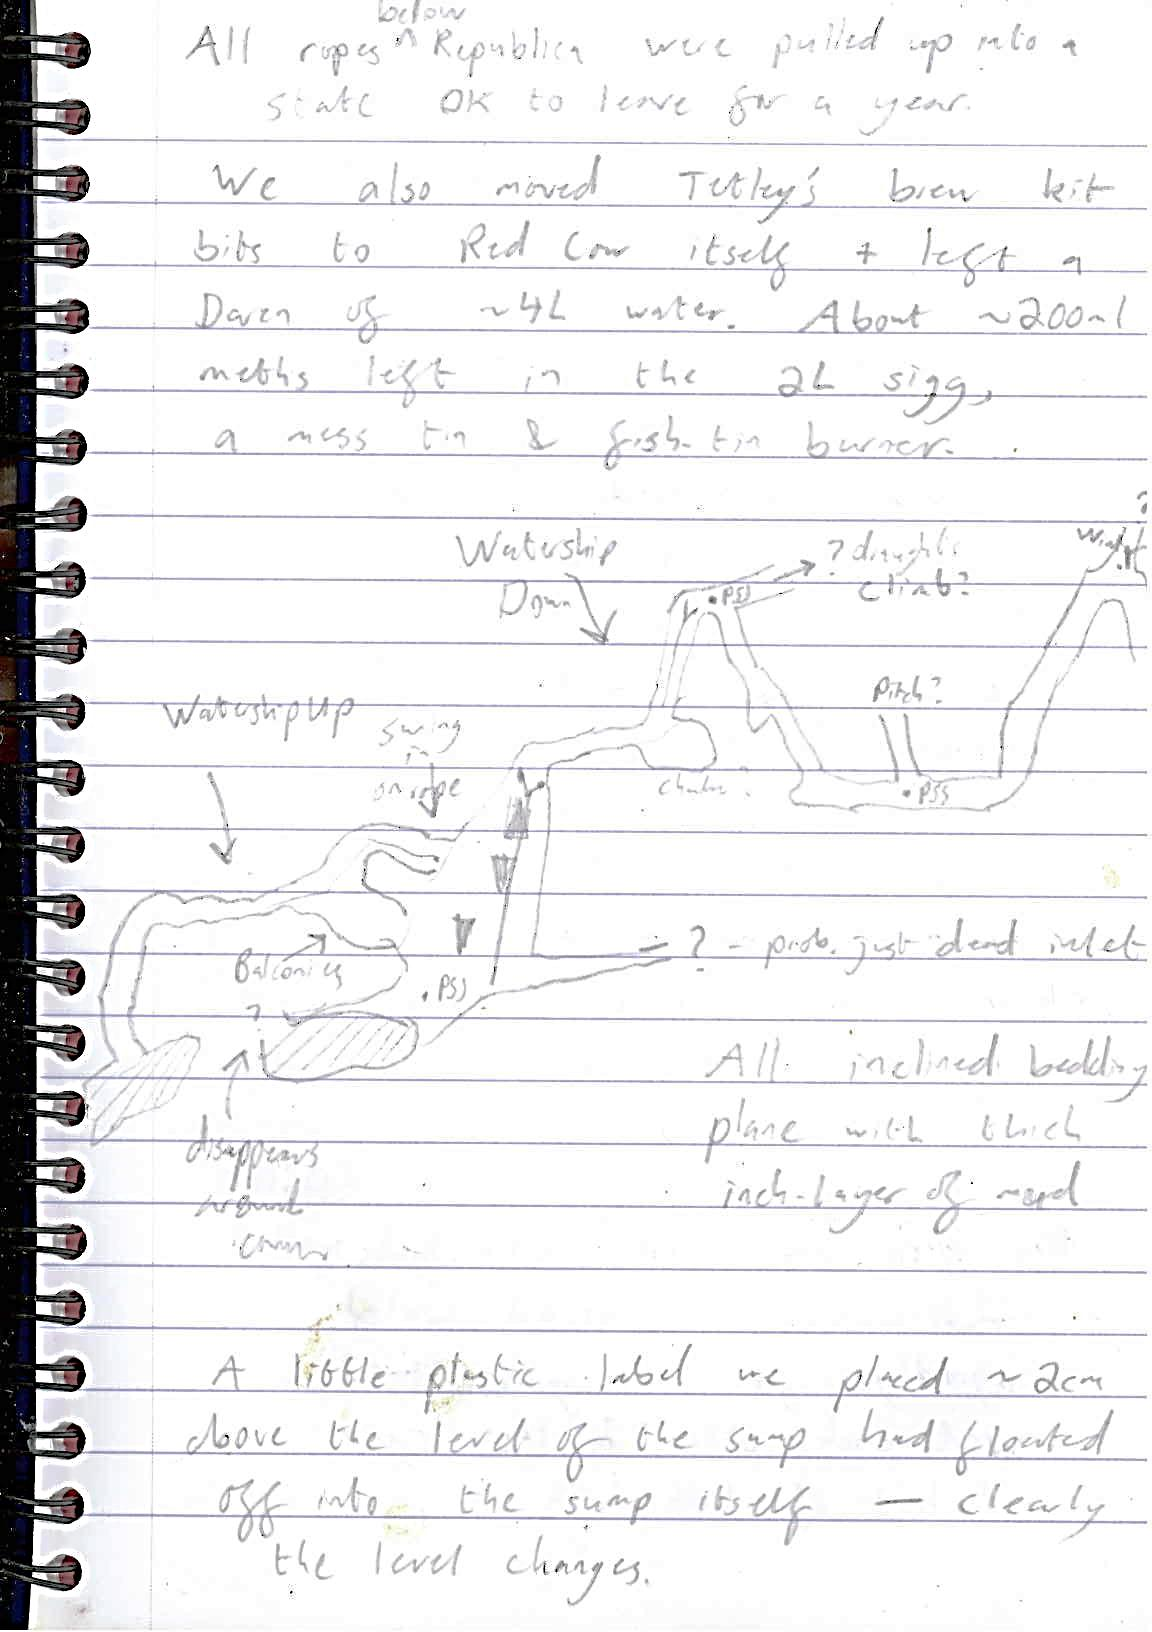
\includegraphics{appendices/ug_logbook/86.jpeg}\\
{[}Jarv's sketch of Watership Up{]}

A little plastic label we placed \textasciitilde 2cm above the level of
the sump had floated off into the sump itself -- clearly the level
changes.

So about to leave \emph{X-Ray} \& the expedition.

A pity the diving didn't work out -- perhaps some other time. I think an
attack on the Watership Down sump will require a capable \& committed
team of Four with a week-fortnight to dedicate.

As part of this I think taking 100 m of rope \& a drill to protect all
the climbs in Leprecaun/Memory lane, setting a proper camp at Red Cow \&
rerigging \emph{Republika} + \emph{Insomnia} (the terrible twins) in a
suitably safe fashion will be necessary steps. This is all obviously
rather far-fetched on a student expedition where everyone has their own
plans \& intrigues.

So goodbye for this year -- respect each other \& the cave, and best of
luck with all your pushes.

\textbf{4/8/12 10 a.m. Tetley}

26 hrs after waking up (on the surface) I'm making final preparations
before sleep, drinking Long John and writing this. It's been a long day,
but a great one. \emph{Brave New World} goes! Squeezed through boulder
choke to reach \emph{Invictus} -- 70 odd metre of very fine sandy
passage ending in a wet pitch. About 20 m to floor\ldots{}. Left
unpushed does the draught go up it or down it? Slow journey back,
deliberately so not to disturb day train. Sleep now, at last!

\textbf{00:02 5/8/12 Tetley}

Tetley + Rhys have gone to push below \emph{Lower Pleasures}. Callout:
11 a.m.

\textbf{5/8/12 10:30 Dan}

Great day yesterday finished the traverse to Big Rock's big brother.
Very wet, quite sketchy but really fun. There's a new way up from the
bottom of Big Rock, so no one needs to go there again. Except to derig
it The pitch on the other side is huge. We didn't get very far down,
there's \textasciitilde 60 m of 9 ½ at the top for someone else to
enjoy. To the surface!

\textbf{5/8/12 11:00} \textbf{am} \textbf{Rhys}

Back for second night at camp. Strange day, I didn't think Tetley or I
appreciated how knackered we were from our \emph{Brave New World} push.
We started off with the idea of pushing \emph{Yorkshire} but once into
Lower Pleasures we couldn't work out where Oli and Thara had gone. We
ended up bolting down a small waterfall at the bottom of the big
\emph{Lower Pleasures} pitch. We found an incredibly twatty immature
streamway and decided to get out because it was so rubbish. We then did
a tourist trip to Cactus Junction and \emph{the Fridge} camp, which was
really nice to see. Also looked at the Big Rock parallel shaft that Dave
and Dan were pushing. There's some heroic bolting there to get to what
looks like (and sounds like) a reasonably big pitch. Hoping to sleep for
a while and head out early Monday morning.

\textbf{5/8/12 18:00 Tetley}

Left at HAWAII (junction below Stuck in P.)

1 empty fish tin (a.k.a. meths stove!)

1 mess tin

1 daren drum full of water (can refill by placing under drips at bottom
of \emph{Stuck in Paradise})

600 ml of meths

N.B. There is NO lighter there -- Bring one if you want hot water!

\textasciitilde 20 m of yellow rope

% \begin{center}\rule{0.5\linewidth}{\linethickness}\end{center}

Climb in \emph{Brave New World} now rigged using \textasciitilde 40 m
rope length (only about 8 m is actually needed for this). Suggestion:
rerig climb using short rope and use the 40 m length for exciting pitch
at end of \emph{Invictus}.

\textbf{5/8/12 21:00 Tetley}

Consciousness is slipping away again. We've been awake for 3 ½ hrs,
watched Withnail and I, and Red Dwarf. Only Rhys and I here, now back to
sleep hopefully.

\textbf{6/8/12 7:00 a.m. Tetley}

Excellent, another 9 hrs in bed! Feel well rested, Van Morrison's
`Gloria' blasting out on the stereo, a big pot of tea is in front of
me\ldots{}.. life is good!

\textbf{6/8/12 7:20am Rhys}

Why is camp downwind of the shit area? Why?!

\textbf{6/8/12 8:20 a.m. Tetley}

Another meal of cheesy, soupy, fishy, smash. Classic! Only pepper
missing, I can see what drove the spice trade.

\textbf{6/8/12 10 a.m. Tetley}

We're off to the surface. Thanks Rhys for another great weekend in the
underground. Good pushing all!

\textbf{7/8/12 8:30} \textbf{am} \textbf{Thara}

Tim and I (dreamt team) went for the glory at Big Rock (soon to be
called \emph{Stagger Lee}). After arriveing at the camp around 830pm,
faffed around cooking, eating, drinking. We soon found that the camp was
without a drill bit.

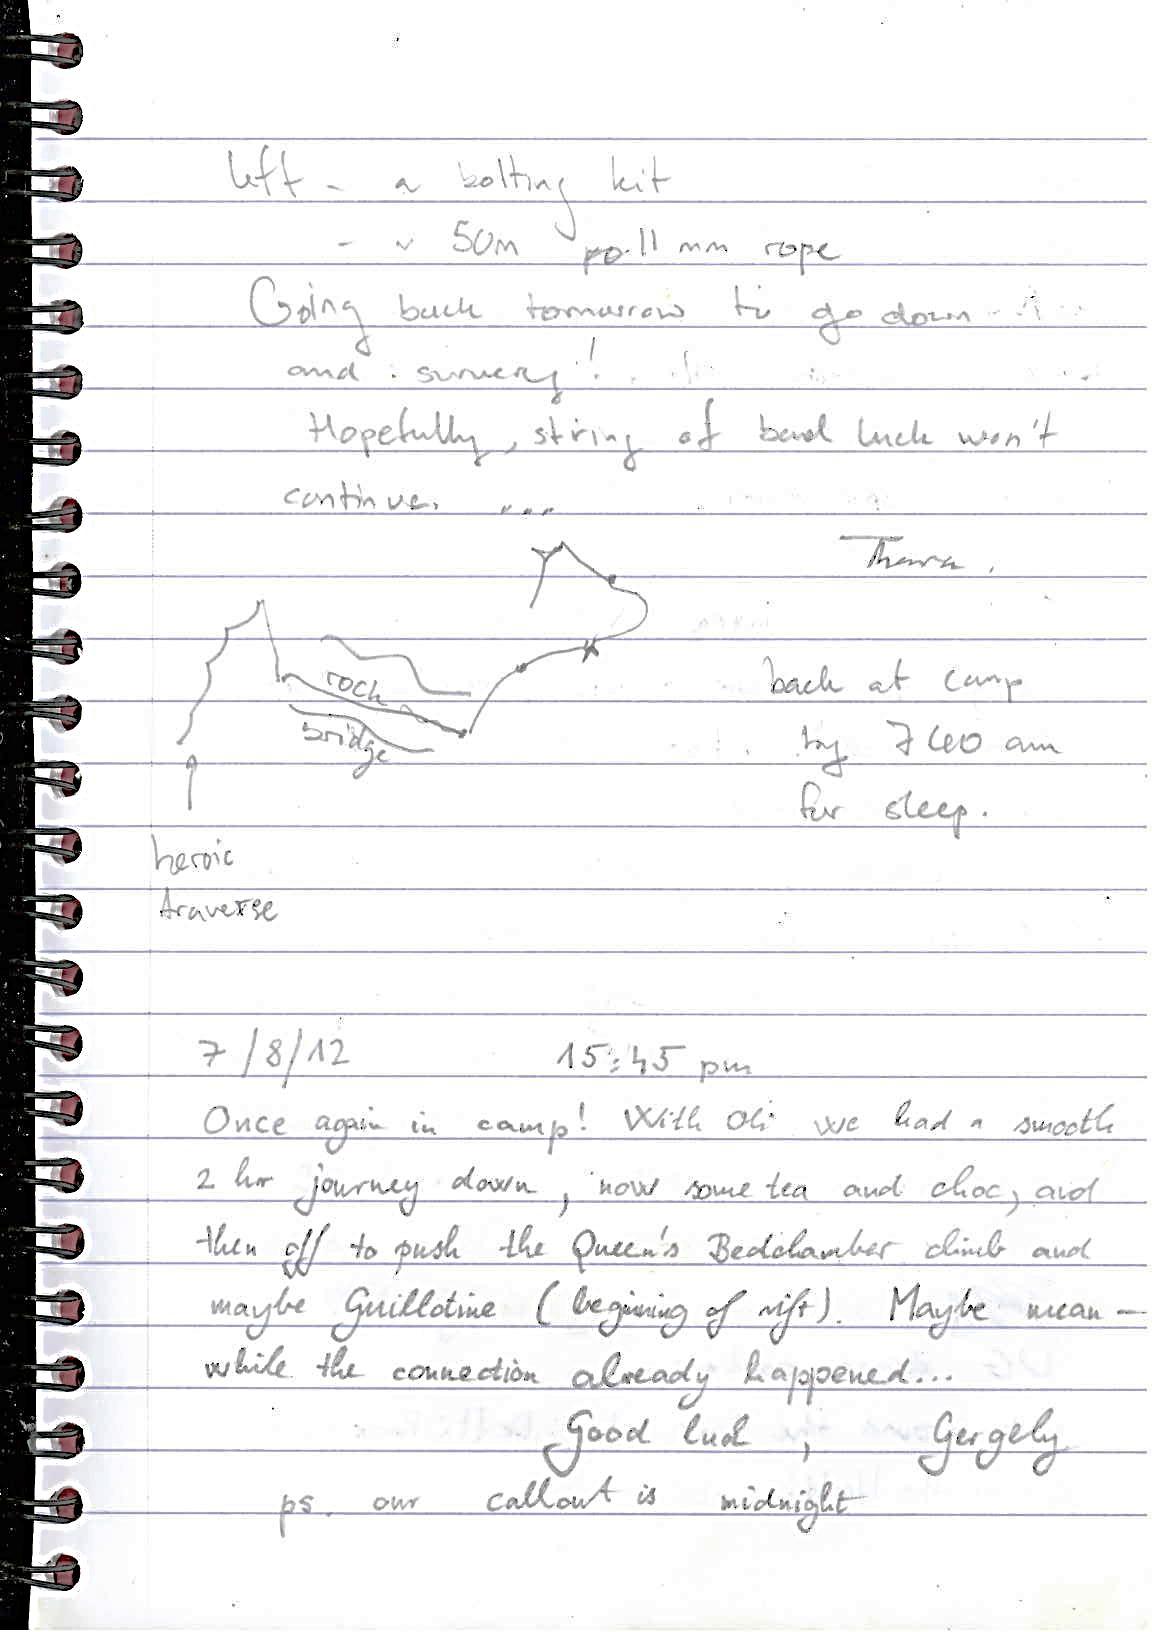
\includegraphics{appendices/ug_logbook/87.jpeg}Nevermind, old style bolting mission.
Set off around 10pm to Big Rock. After the first bolt we soon have a
fucked driver. Rock here was pretty, two bolts wasted as a proceed.
However we managed to bolt down to the second level, where Tim braved
the drizzle (like \emph{Zimmer}) and tried to bolt down to the lower
level.

Left

\begin{itemize}
\item
  a bolting kit
\item
  \textasciitilde 50 m 11 mm rope
\end{itemize}

Going back tomorrow to go down and survey!

Hopefully, string of bad luck won't continue\ldots{}

{[}Thara's sketch of Big Rock traverse {]}

\textbf{7/8/12 15:45 pm Gergely}

Once again in camp! With Oli we had a smooth 2 hr journey down, now some
tea and choc, and then off to push the Queen's Bedchamber climb and
maybe Guillotine (beginning of rift). Maybe meanwhile the connection
already happened\ldots{}

Good luck, Gergely

ps. our callout is midnight

\textbf{7/8/12 JONNY (+ KATE) 23:00}

Nice trip down to camp before going to push Euphrates. Really shit rock
-- 4 attempted bolts + lots of broken rock. However, super strong draft
+ the pitch looks very promising.

! GO BACK ! (someone, not me\ldots{})

Surveying was a pain (cold, muddy, shit) BUT -- Euphrates is now tied in
which is v. satisfying.

Looking forward to pushing elsewhere tomorrow.

UG dance routine:

Walk around the tent to Daft Punk's Around the World!

\textbf{7/8/12 JONNY 00:30}

OLI on tacklesacks:

``It's good, it's like walking with a massive cock in my hand

Me on people not missing their callouts:

``Good, I can take off my furry''

\textbf{8/8/12 1:45 Gergely}

Pushing Queen's Bedchamber was great; put in \textasciitilde 12 bolts,
now we are at the bottom of the rift, and \textasciitilde 8 m higher the
end of a phreatic can be seen (maybe?) PLUS everything is covered w
black dust, as the beginning of King Minos palace! It really looks
exciting. Altogether \textasciitilde 30 bolts in the climb so far, one
more session needed.

Whisky is good.

\textbf{8/8/12 3 pm Gergely}

Tim \& Thara just got back from connection to Soda stream. Olli \& me
are about to set off to \emph{Minestrone}, trying the connection to
Balamory. Our callout is 10am on Thursday. Kate is still hesitating but
probably she and Jonny are going to come to the \emph{Atlantis} area as
well.

\textbf{8/8/12 4pm Thara}

Officially, we (Tim and I) are the connection makers (loopers).

We surveyed from the bottom Big Rock b/c we couldn't find any Pss
station. Hopefully, we make a connection at the right place there.

\begin{itemize}
\item
  Bottom of Big Rock Rope
\item
  A pile of spitzes (\textasciitilde 3)
\end{itemize}

Continued bolting down the pitch, Dan planned to descend. Tim put two
quick bolts (thanks to drill bit) and dropped down to the bottom which
is filled with human-size boulders stacked Jenga-like.

We looked for the obvious chamber by following the streamway.

3 bolts and we were at the bottom followed the stream for a few more
minutes until we realised that we were in Soda Streamway -- CONNECION!
Again.

Slow surveyed the rest and derigged all the ropes.

3 possible leads (Not that exciting)

\begin{enumerate}
\def\labelenumi{\arabic{enumi}.}
\item
  Window at the same lvl as rock wall
\item
  Window at the same lvl as traverse ledge
\item
  Window \textasciitilde 3 metres above the bottom
\end{enumerate}

The first two seem to head back into the rifts already explored. The
third seems to head towards Balimory.

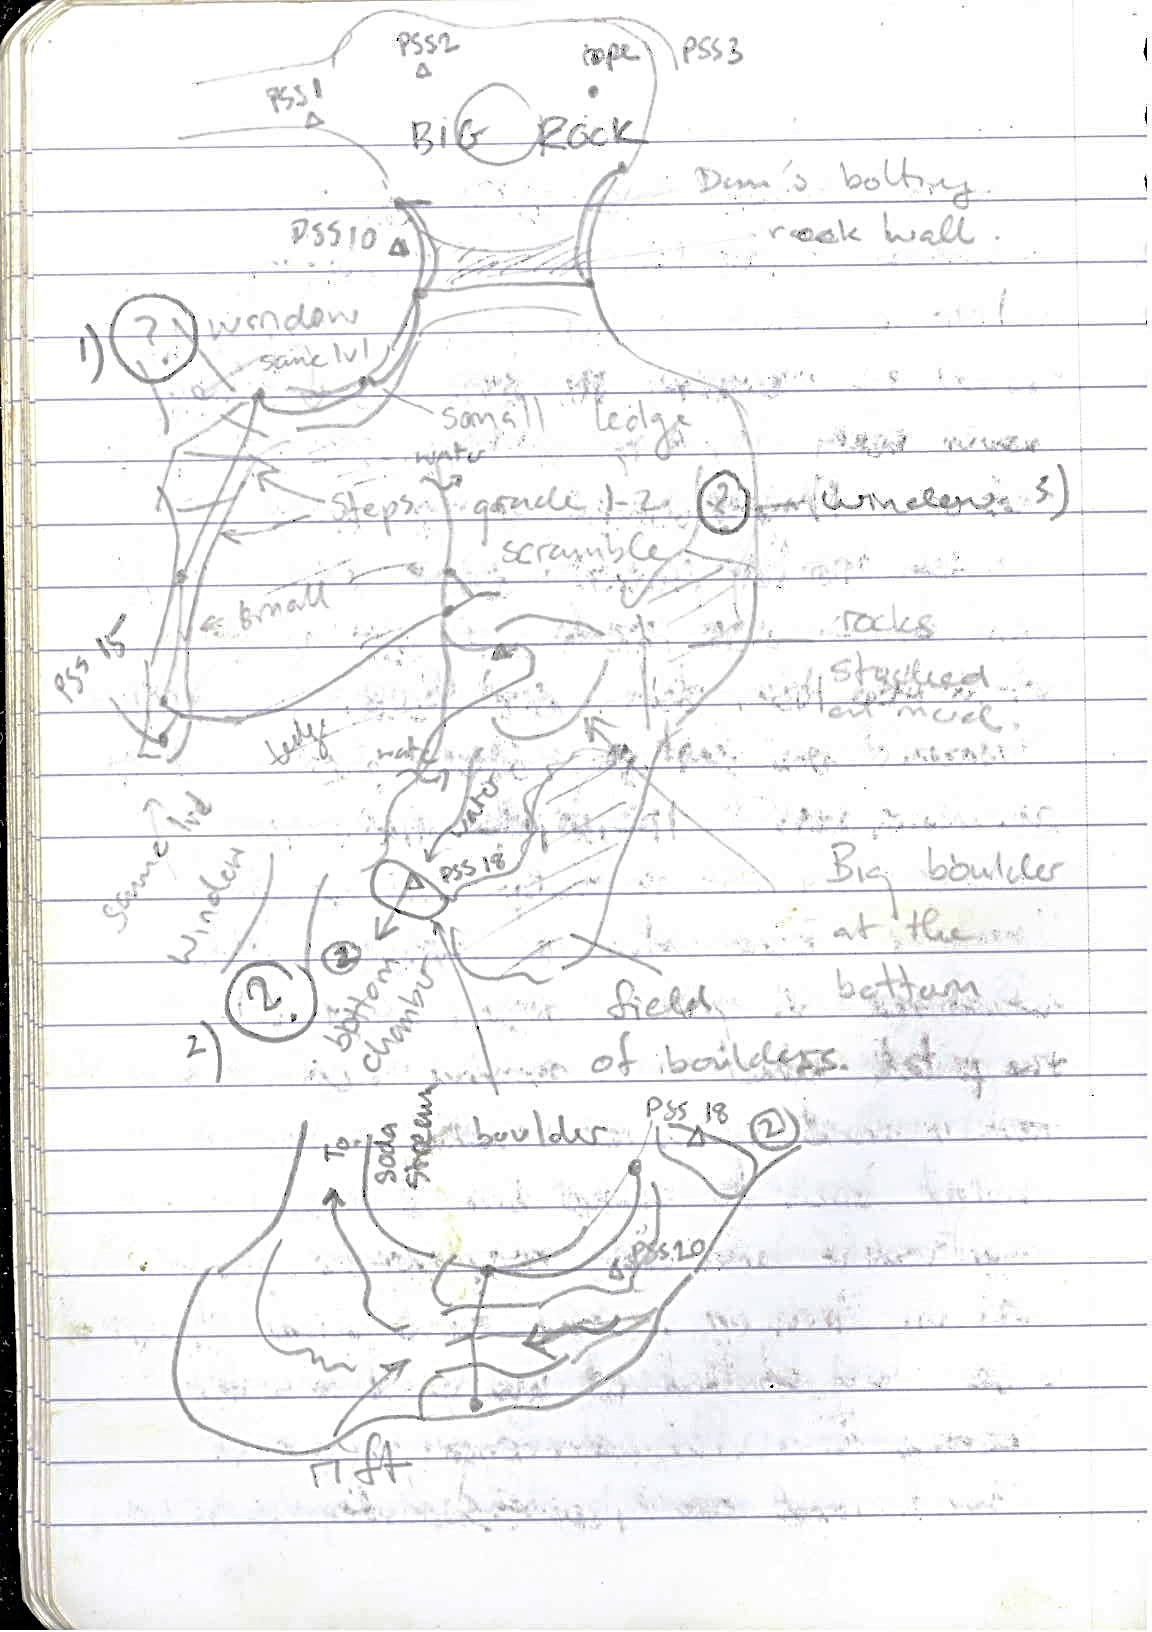
\includegraphics{appendices/ug_logbook/88.jpeg}\\
{[}Thara's sketch of Big Rock, with leads {]}

\textbf{8/7/12 16:45 Kate}

Well, Jonath and myself set off from the Bivi yesterday and I realised
at the entrance that I just wasn't that keen, we set off anyway thinking
that I was being silly and the enthusiasm would soon set in.
Unfortunately in the Urinal Series the fun had not begun, dear dear
Jonath was lovely and made me feel ok so we got to the big pitches and
things got better. It wasn't any sort of extreme fear, just an
unwillingness to be in the fun caving state. We eventually got to camp
and set off to Xanadu/Euphrates to connect the survey which was v. grim.
Jonny tried to bolt the pitch which is v. blowing \& cold but the rock
is shit and kept breaking. We headed back to camp but I still wasn't
comfortable and was very shaky. After lots of dancing, which me \&
Jonath happened to be very skilled at, we went to bed. Today I wasn't
keen to go as far as \emph{Atlantis} but really wanted to for Jonny so
just as we were about to set off Jonny realises that he's also raptured
and just wanted to head out. Much to Gergely's confusion we realised
that neither of us were super enthused then we should cut our losses and
head out, freeing up bed space for the mega-keen. We still accomplished
the Xanadu/Euphrates connection and have had a pleasent time. We shall
definitely be coming back super-pumped and ready for action, just this
time wasn't meant to be.

Peace out

Kate x

Besides I quite need a shit and I have sworn to never poo underground.

\textbf{9/8/12 Thara 8:40} \textbf{am}

After two pushing trip, it is time to head up again. Have a good one!

\textbf{9/8/12 Gergely 8:45} \textbf{am}

We were badly defeated by the Almighty Chokes. Fighting w 2 today, the
\emph{Minestrone} one seems to fill up the whole passage; the Inglorious
Basterd (starting at pitch at \emph{Atlantis}/\emph{Minestrone}) seems
to be more pushable, but we ran out of time \& enthusiasm. Spent cca 7
hours digging. Now time for sleep and maybe catch the sunset! Good luck.

\textbf{4:45 pm}

We head off \& hope more dinner is left for us! Good times again, see
you one more time, Camp \emph{X-Ray}!

\textbf{10/8/12 Erik/Matjer/Maffi}

We come to CAMP X RAY 00.30 sleep

8.00 we go to Queen CAMBER to climb a {[}illegible{]}. We climbed 20 m
and finde a galerije more than CCA 400 m

We don't measure because of time.

In the end is a big chamber in wather is coming down. The gallery is
very muddy. In the end where is a chamber is a hole down cca 30 m where
the wather is going. Now we are going out.

\textbf{10/08/12 9:50 pm Sam}

SO happy to be back -- finally. Was apprehensive about coming down after
the adventures of last time -- both coming down and going out turned
into mini epics, but coming down today just took us 2 ½ hours. Compared
to last time's 5 hourish trip down, this felt like such a jolly. The 5
hours were due to an hour stuck at the top of skynet and another hour on
\emph{Zimmer}'s rebelays, but the rebelays posed to problem today. I was
fully expecting to have to faff with footloops etc to pass the rebelays,
but no such thing was needed. Camp is as homely as I remember.

We passed the 3 Slov's coming up at Tesalator -- they had found a lot of
horizontal passage ending in a pitch; all of which they hadn't surveyed.
Can't remember where they had gone -- I'm sure Clare will write in more
detail. We're both interested in seeing and surveying the stuff they
have found -- probably tomorrow's mission. I think it will be good to do
more surveying -- apparently the novelty wears off however\ldots{}

\textbf{10/8/12 10:55 PM Clare}

Enjoying my first ever cigarette at UG camp while listening to Lou
Reed's Walking on the Wild Side -- a momentous occasion! Great to be
back at \emph{X-Ray}, almost forgot how much I love underground camp
after being distracted by M2 for the past week. Just Sam and I here now.
Whisky + Blackadder then bed.

\textbf{11/8/12 10:52 AM Clare}

Sam and Clare off to Queen's Bedchamber. Back by 2AM, 12/8/12.

\textbf{11/8/12 11:09 PM Clare}

Great day of pushing! Surveyed the passage found by Eric \& co. and
pushed some new stuff. Almost 500 m in the book! Named the bolt climb
\emph{Apollo} (as suggested by Gergely), and the horizontal stuff after
that is MILKY WAY. Three main leads in Milky Way -- two pitches and one
wide open horizontal virgin passage (!!).

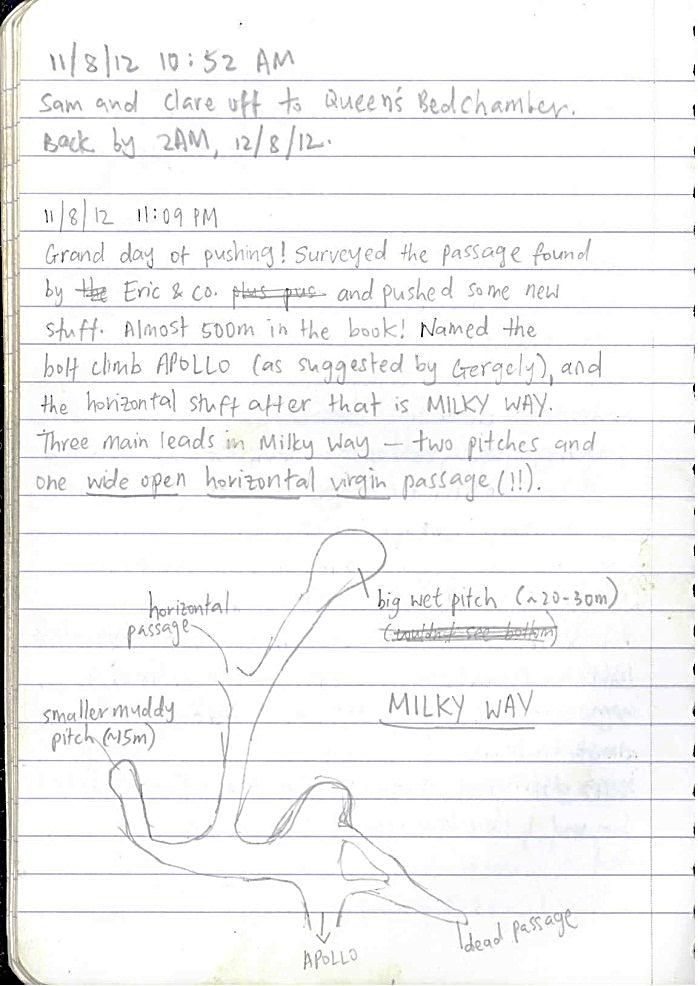
\includegraphics{appendices/ug_logbook/89.jpeg}\\
{[}Clare's map of Milky Way {]}

\emph{Apollo} was a super bolt climbing effort by Gergely, Izi, Maver
and Eric! It's like \emph{Cheetah}/\emph{Stuck in Paradise} in reverse.
Good to see their efforts have paid off with so much passage.
Immediately after \emph{Apollo} is a shitty handline/pitch climb down a
muddy slope. Belays aren't great so take care!

Now in bed ensconced in TWO nitestars.

\textbf{12/8/12 9:20 AM Sam}

Had a great day yesterday. Clare mentioned that the amount of surveying
we did yesterday may be a record for a virgin surveyor. Hmm\ldots{} data
will reveal all, but it definitely felt like a lot of surveying! Did get
a bit fed up with using the instruments towards the end. But the stuff
we found was very exciting -- and there are existing leads that we left.
Today, we are heading out. Should be ok -- long but it needs
doing\ldots{}

\textbf{12/9/12 9:25 AM Clare}

Maffi and Tjasa are here on the night train! They bottomed the big wet
pitch at end of Milky Way, leads to a narrow rift that's still going.
It's been a fantastic camp, can't wait to be back next year!

\textbf{13.8.12 Tjasa}

We were at the end of Milkyway bolting the pitch. And everytime when we
are together in the cave we find some rifts

Then we woke up and it was around 3 at night. First we were confused and
then we realized that nobody comes in to the camp. We were a bit late to
go back to the end of the Milkway so we decided to wait until somebody
comes inside, we thought that that will be at 9 in the morning. But now
its 10\textsuperscript{30} and still nobody here.

Now: drinking tea, not knowing what to do \& wondering what's going on
outside\ldots{} it's pretty same every year at the underground camp

Aja: hvala za dobr kamp!

\textbf{13.8.12 Maffi}

I don't know what to hope: That this underground adventures with Tjasa
will become a tradition or not! Like last year (my first time down here)
we found the narrowest and the longest wet passages possible again. But
those places are also so beautiful, that I hope someone will discover
big chambers with a lot of new leads on the other side, and meabe a
shortcut to get there , so many of you will have the motivation to go
there and see what we saw! For those of you who want, I'll try to draw a
picture:

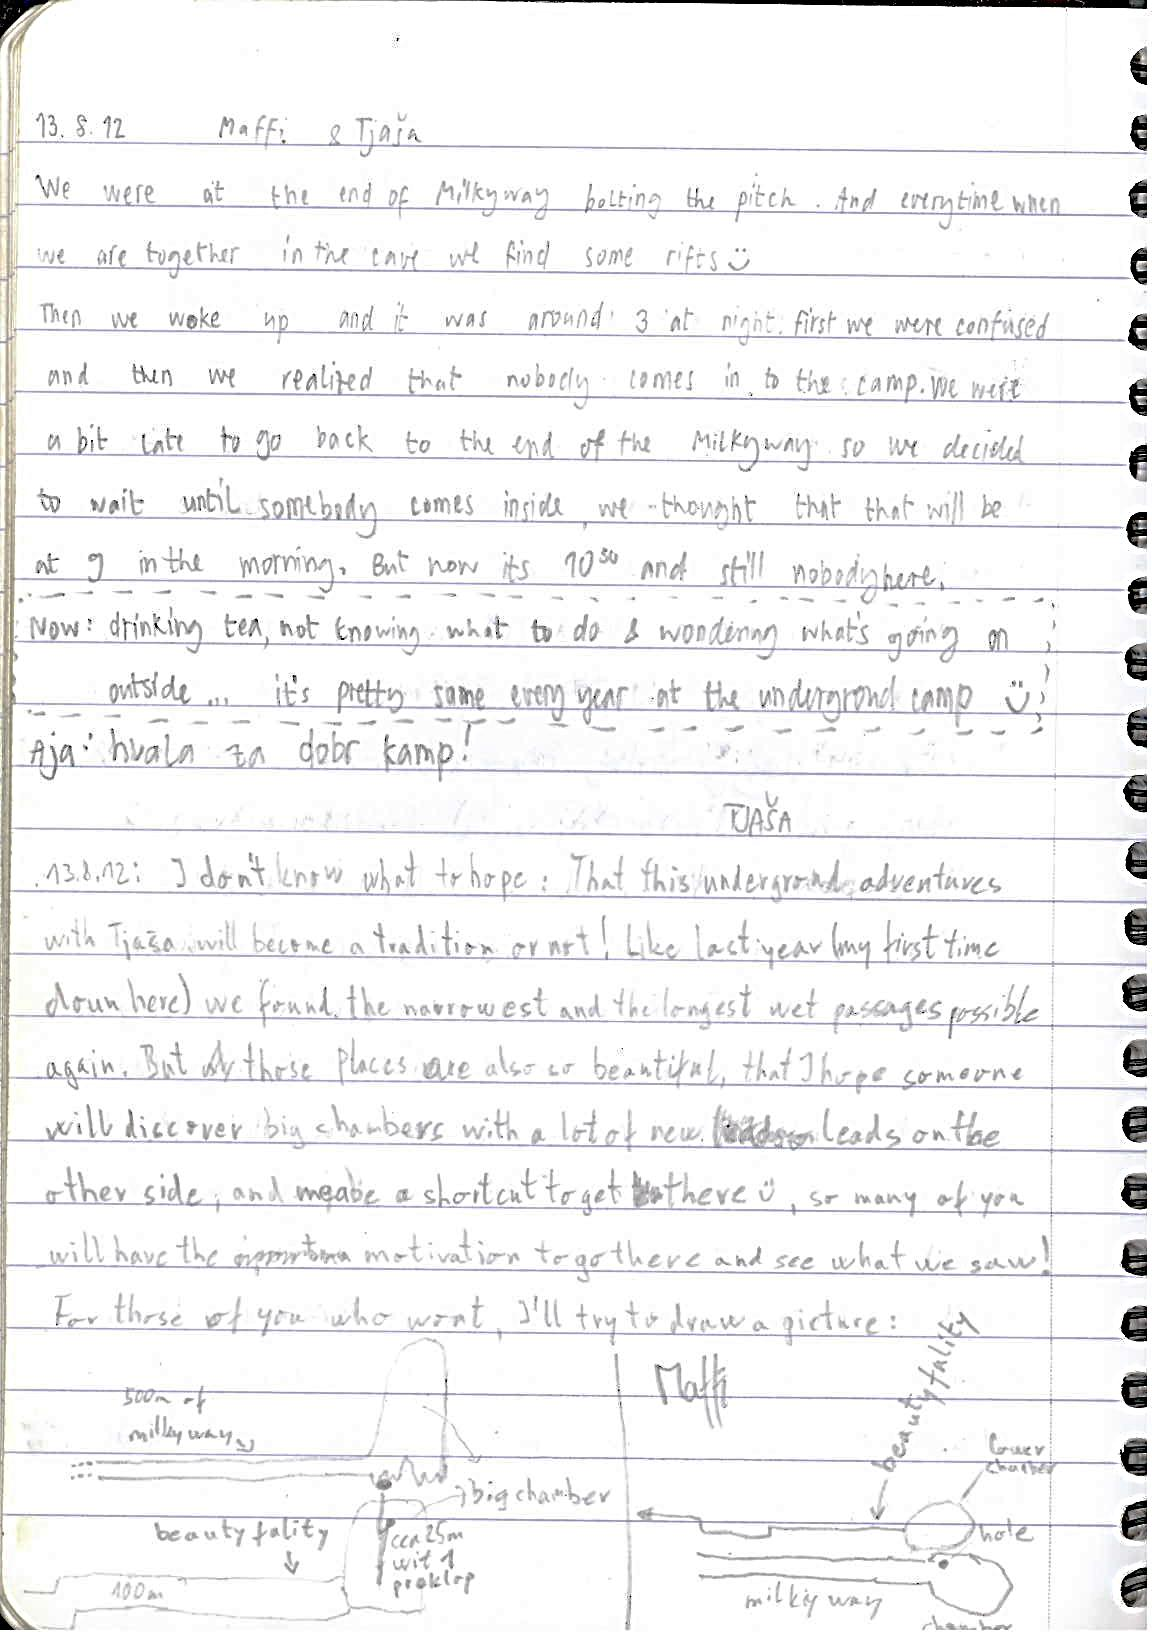
\includegraphics{appendices/ug_logbook/90.jpeg}\\
{[}Maffi's sketch of pitch at end of Milky Way {]}

\textbf{14/8/2012 1:15 am Karin}

Long John time! We deserved it, we pushed the \emph{Vrtnarija} for 70 m
(that's what Gergely said) down That means also that we found around
12km ``new'' cave -\textgreater{} it has a name -\textgreater{} Sistem
Migovec. I still can't believe it.

We wanted to bolt to the right window in Queen's Bedchamber, but the
drill broke. That's why we went up left into Milky Way to check out the
unpushed passage. The direction and draft (+ cristals ) were showing us
that we'll get somewhere near Sistem. But we didn't expect that we're
going actualy find the connection. Gergely said that we had luck. For a
few moments I also belived so (that's when I saw the PSS13 -- Waterloo)
but I don't belive in luck, OK there is possibility that we had luck,
but that's just a rare moment when you can't explain it differently than
saying it was luck (if you ask me). However I don't care what it was, we
found the connection and both of us are very happy .

Aja! I forgot, we called the passage Dreams for the Soul (or in SLO:
Sanje Za Duso) LP!

\textbf{Gergely}

Once upon a time, a black and a red furry went down to a cave and came
out at -70.

So today everything worked out like in a perfect fairy tale. We wanted
to climb, but the dwarves broke the cable. Then we followed the crystals
which eventually led to the hidden treasure: a bolt in the wall!
Waterloo is a nice chamber. We also found the continuation of
Guillotine/Minotaur rift. What a glorious end to this successful expo!
The connection is a proper teamwork, and we happened to be the lucky
ones, a great honor from \emph{Vrtnarija}\ldots{}

Now it is only 2 of us + the hot choc whiskey in the cave. Candle lit
dinner and happy times. It is like ahome in the mountain. All the best
until next year!

p.s. hot choc w whiskey is a great recipe!

\textbf{14/8 1pm Gergely}

The morning I felt absolutely shit, probably Karin illness My stomach is
still not too good, hopefully no problem on way out. Happy cavers emerge
from Friendship Gallery, packing up starts, it will be hard to go
out\ldots{} But everything is illuminated by the Connection! Good-bye
until next year, Gergely.

\textbf{14/8 1pm Jonny}

So, an ordinary derig was made much less ordinary when Gergely + Karin
told me that the cave is now 70 m deeper. Hooray for sys-mig.
